% Filename: camecc_lic.tex
% This code is part of 'Cursos CAMECC: Introducao ao LaTeX para o Curso 29 - Licenciatura em Matematica'
% 
% Description: This file correspond to the textbook using in the course.
% 
% Created: 07.06.12 11:30:10 AM
% Last Change: 26.06.12 11:07:21 PM
% 
% Authors:
% - Raniere Silva, r.gaia.cs@gmail.com
% 
% Organization: CAMECC - Centro Academico dos Estudantes do IMECC
% 
% Copyright (c) 2012, Raniere Silva. All rights reserved.
% 
% This work is licensed under the Creative Commons Attribution-ShareAlike 3.0 Unported License. To view a copy of this license, visit http://creativecommons.org/licenses/by-sa/3.0/ or send a letter to Creative Commons, 444 Castro Street, Suite 900, Mountain View, California, 94041, USA.
%
% This work is distributed in the hope that it will be useful, but WITHOUT ANY WARRANTY; without even the implied warranty of MERCHANTABILITY or FITNESS FOR A PARTICULAR PURPOSE.
%
\documentclass[12pt,a4paper,openright,twoside]{book}
\usepackage[top=3cm,left=2cm,right=2cm,bottom=3cm]{geometry}
\usepackage[brazil]{babel}
\usepackage{indentfirst}
% Filename: package.tex
% This code is part of 'LaTeX with Vim'.
% 
% Description: This file correspond to the packages to be used.
% 
% Created: 07.06.12 11:30:10 AM
% Last Change: 26.06.12 11:07:21 PM
% 
% Authors:
% - Raniere Silva, r.gaia.cs@gmail.com
% 
% Copyright (c) 2012, Raniere Silva. All rights reserved.
% 
% This work is licensed under the Creative Commons Attribution-ShareAlike 3.0 Unported License. To view a copy of this license, visit http://creativecommons.org/licenses/by-sa/3.0/ or send a letter to Creative Commons, 444 Castro Street, Suite 900, Mountain View, California, 94041, USA.
%
% This work is distributed in the hope that it will be useful, but WITHOUT ANY WARRANTY; without even the implied warranty of MERCHANTABILITY or FITNESS FOR A PARTICULAR PURPOSE.
%
\usepackage[utf8]{inputenc}
\usepackage[T1]{fontenc} 
% \usepackage[top=3cm,left=2cm,right=2cm,bottom=3cm]{geometry}  % Set in the file.
% \usepackage[brazil]{babel}  % Set in the file.
% \usepackage{indentfirst}  % Set in the file.

% Text
\usepackage{enumerate}
\usepackage{latexsym}
\usepackage{parcolumns}
\usepackage[hyphens]{url}
\usepackage{hyperref}
\usepackage{breakurl}
\usepackage[official]{eurosym}

% Tables
\usepackage{multicol}
\usepackage{multirow}
\usepackage{array}

% Math
\usepackage{amsthm}
\usepackage{amsmath}
\usepackage{amsfonts}
\usepackage{amssymb}

% Index
\usepackage{makeidx}
\makeindex

% Figures
\usepackage{pb-diagram}
\usepackage{graphicx, color}
\usepackage{subfig}
\usepackage{tikz}
\usetikzlibrary{patterns}
\usepackage{epsfig}

% Algorithm
\usepackage{algorithmic}
\usepackage{algorithm}
\usepackage{listings}
\usepackage{listingsutf8}

% New commands and enviromments
\newcommand{\TikZ}{Ti\emph{k}Z }
\newcommand{\PGF}{\textsc{PGF} }
\newcommand{\flang}[1]{\textit{#1}}

\lstset{
language=TeX,
basicstyle=\ttfamily,
showspaces=false,
showstringspaces=false,
showtabs=false,
tabsize=2,
breaklines=true,
breakatwhitespace=false,
}
\newcommand{\lcode}[1]{\lstinline!#1!}  % Code in the same line. Deprecated: limitations to handle with backslash and curly brackets. 
\newcommand{\envname}[1]{\lstinline!#1!}  % Name of environments.
\newcommand{\pkgname}[1]{\lstinline!#1!}  % Name of environments.
% Name of commands use \lstinline!\command_name!.
\lstdefinestyle{example}{
language=TeX,
basicstyle=\ttfamily\footnotesize,
showspaces=false,               % show spaces adding particular underscores
showstringspaces=false,         % underline spaces within strings
showtabs=false,                 % show tabs within strings adding particular underscores
tabsize=2,                      % sets default tabsize to 2 spaces
breaklines=true,                % sets automatic line breaking
breakatwhitespace=false,        % sets if automatic breaks should only happen at whitespace
escapeinside={\%}{\^^M},
aboveskip=-12pt,
}
\renewcommand{\lstlistingname}{C\'{o}digo}
\lstnewenvironment{code}[1][style=example,]{}{}  % Code in new line.
\newcommand{\fcode}[1]{\lstinputlisting[style=example,]{#1}}  % Code in a file.
\newcommand{\example}[1]{  % For examples.
\begin{minipage}[c]{0.5\textwidth}
    \fcode{#1}
\end{minipage} \quad \vrule \quad
\begin{minipage}[c]{0.35\textwidth}
    \input{#1}
\end{minipage}
}
\newcommand{\examplebeamer}[1]{  % For examples.
\begin{minipage}[c]{0.5\textwidth}
    \fcode{#1}
\end{minipage} \quad \vrule \quad
\begin{minipage}[c]{0.35\textwidth}
    \fbox{\includegraphics[width=\textwidth]{#1}}
\end{minipage}
}

\begin{document}
\title{Cursos CAMECC \\ Introdu\c{c}\~{a}o ao \LaTeX \ para o Curso 29 \\ Licenciatura em Matem\'{a}tica}
\author{Raniere Silva}
\maketitle

% Frontmatter
\frontmatter 

% Filename: licence@cammec_lic.tex
% This code is part of 'Cursos CAMECC: Introducao ao LaTeX para o Curso 29 - Licenciatura em Matematica'
% 
% Description: This file correspond to the licence of the textbook using in the course.
% 
% Created: 07.06.12 11:30:49 AM
% Last Change: 07.06.12 11:30:53 AM
% 
% Authors:
% - Raniere Silva, r.gaia.cs@gmail.com
% 
% Organization: CAMECC - Centro Academico dos Estudantes do IMECC
% 
% Copyright (c) 2012, Raniere Silva. All rights reserved.
% 
% This work is licensed under the Creative Commons Attribution-ShareAlike 3.0 Unported License. To view a copy of this license, visit http://creativecommons.org/licenses/by-sa/3.0/ or send a letter to Creative Commons, 444 Castro Street, Suite 900, Mountain View, California, 94041, USA.
%
% This work is distributed in the hope that it will be useful, but WITHOUT ANY WARRANTY; without even the implied warranty of MERCHANTABILITY or FITNESS FOR A PARTICULAR PURPOSE.
%
\section*{Licen\c{c}a}

Este trabalho \'{e} baseado em:
\begin{itemize}
    \item ``LaTeX com Vim (e Git)'' de Raniere Silva, licenciado com a Licen\c{c}a Creative Commons Atribui\c{c}\~{a}o - CompartilhaIgual 3.0 N\~{a}o Adaptada (\url{http://creativecommons.org/licenses/by-sa/3.0/}) e dispon\'{i}vel em \url{https://github.com/r-gaia-cs/latex_with_vim/};
    \item ``TikZ para professores'' de Raniere Silva, licenciado com a Licen\c{c}a Creative Commons Atribui\c{c}\~{a}o - CompartilhaIgual 3.0 N\~{a}o Adaptada (\url{http://creativecommons.org/licenses/by-sa/3.0/}) e dispon\'{i}vel em \url{https://github.com/r-gaia-cs/latex_with_vim/}.
\end{itemize}

Salvo indica\c{c}\~{a}o em contr\'{a}rio, este trabalho foi licenciado com a Licen\c{c}a Creative Commons Atribui\c{c}\~{a}o - CompartilhaIgual 3.0 N\~{a}o Adaptada. Para ver uma c\'{o}pia desta licen\c{c}a, visite \url{http://creativecommons.org/licenses/by-sa/3.0/} ou envie um pedido por carta para Creative Commons, 444 Castro Street, Suite 900, Mountain View, California, 94041, USA.

%The photo X is © 2009 Jane Park, used under a Creative Commons Attribution-Noncommercial license: http://creativecommons.org/licenses/by-nc/3.0/.
\begin{center}
    
\includegraphics[keepaspectratio=true]{../../figures/cc-by-sa.png}
\end{center}


% Preface
% Filename: preface@cammec_lic.tex
% This code is part of 'Cursos CAMECC: Introducao ao LaTeX para o Curso 29 - Licenciatura em Matematica'
% 
% Description: This file correspond to the preface of the textbook using in the course.
% 
% Created: 07.06.12 11:30:49 AM
% Last Change: 07.06.12 11:30:53 AM
% 
% Authors:
% - Raniere Silva, r.gaia.cs@gmail.com
% 
% Organization: CAMECC - Centro Academico dos Estudantes do IMECC
% 
% Copyright (c) 2012, Raniere Silva. All rights reserved.
% 
% This work is licensed under the Creative Commons Attribution-ShareAlike 3.0 Unported License. To view a copy of this license, visit http://creativecommons.org/licenses/by-sa/3.0/ or send a letter to Creative Commons, 444 Castro Street, Suite 900, Mountain View, California, 94041, USA.
%
% This work is distributed in the hope that it will be useful, but WITHOUT ANY WARRANTY; without even the implied warranty of MERCHANTABILITY or FITNESS FOR A PARTICULAR PURPOSE.
%
\chapter{Pref\'{a}cio}
Esse mat\'{e}ria foi desenvolvido para um mini-curso voltados aos aulos do curso de Licenciatura em Matem\'{a}tica da Universidade Estadual de Campinas (UNICAMP).

O objetivo do mini-curso \'{e} apresentar o LaTeX aos futuros licenciados em matem\'{a}tica e ajud\'{a}-los a dominar essa poderosa ferramenta de trabalho.

\nocite{LaTeX_Project:EN:Home}Quando me perguntam por que utilizar o LaTeX eu respondo:
\begin{quote}
    \begin{enumerate}
        \item \'{E} uma ferramenta livrer.
        \item \'{E} bastante est\'{a}vel (lan\c{c}ado em 1985 por Laslie Lamport e baseado no TeX que foi lan\c{c}ado por Donald Knuth em 1978).
        \item E possue uma \'{o}tima qualidade tipogr\'{a}fica, i.e., muito bonito.
    \end{enumerate}
\end{quote}
Al\'{e}m dos tr\^{e}s motivos mencionados acima ainda posso dizer que
\begin{itemize}
    \item \'{e}, usualmente, utilizado na produ\c{c}\~{a}o dos mais variados documentos t\'{e}cnico e cient\'{i}ficos,
    \item e encoraja o autor a preocupar-se apenas com o conte\'{u}do.
\end{itemize}

O mini-curso foi preparado para ser ministrado em quatro horas sendo que cada hora deve cobrir um dos cap\'{i}tulos. Al\'{e}m dos cap\'{i}tulos encontra-se no ap\^{e}ndice uma preve hist\'{o}ria de fatos importantes na \'{a}rea de computa\c{c}\~{a}o que ajudam a entender o surgimento do LaTeX, uma explica\c{c}\~{a}o t\'{e}cnica do LaTeX e dicas de locais para procurar ajuda, e alguns exerc\'{i}cios.
 

\tableofcontents 
\listoftables

% Mainmatter
\mainmatter 

% Filename: chap01@camecc_lic.tex
% This code is part of 'Cursos CAMECC: Introducao ao LaTeX para o Curso 29 - Licenciatura em Matematica'
% 
% Description: This file correspond to the chapter 01 of the textbook using in the course.
% 
% Created: 07.06.12 11:30:49 AM
% Last Change: 07.06.12 11:30:53 AM
% 
% Authors:
% - Raniere Silva, r.gaia.cs@gmail.com
% 
% Organization: CAMECC - Centro Academico dos Estudantes do IMECC
% 
% Copyright (c) 2012, Raniere Silva. All rights reserved.
% 
% This work is licensed under the Creative Commons Attribution-ShareAlike 3.0 Unported License. To view a copy of this license, visit http://creativecommons.org/licenses/by-sa/3.0/ or send a letter to Creative Commons, 444 Castro Street, Suite 900, Mountain View, California, 94041, USA.
%
% This work is distributed in the hope that it will be useful, but WITHOUT ANY WARRANTY; without even the implied warranty of MERCHANTABILITY or FITNESS FOR A PARTICULAR PURPOSE.
%
\chapter{Ol\'{a} \LaTeX}
Neste primeiro cap\'{i}tulo apresentamos os conhecimementos m\'{i}nimos de todo usu\'{a}rio do LaTeX. Os cap\'{i}tulos~\ref{sch:history}~e~\ref{sch:get_help} s\~{a}o uma complementa\c{c}\~{a}o a este cap\'{i}tulo podendo ser lidos de maneira independente.

\section{Instala\c{c}\~{a}o}\index{instalacao@instala\c{c}\~{a}o}
Para utilizar o LaTeX voc\^{e} precisa das macros que comp\~{o}em o LaTeX, disponiveis para
\begin{itemize}
    \item Linux: TeX Live\index{TeX Live|see{instala\c{c}\~{a}o}} (\url{http://www.tug.org/texlive}),
    \item Mac OS X: MacTeX\index{Mac OS X|see{instala\c{c}\~{a}o}} (\url{http://www.tug.org/mactex/}),
    \item Windows: proTeXt\index{proTeXt|see{instala\c{c}\~{a}o}} (\url{http://www.tug.org/protext/}) ou MiKTeX\index{MikTeX|see{instala\c{c}\~{a}o}} (\url{http://www.miktex.org/}),
\end{itemize}
e de um editor de texto. \'{E} recomendado que ao inv\'{e}s de um editor de texto utilize-se uma IDE\index{IDE} (\flang{Integrated Development Environment}) pr\'{o}pria para o LaTeX, como
\begin{itemize}
    \item TeXworks\index{TeXworks|see{IDE}} (\url{http://www.leliseron.org/texworks/}),
    \item Kile\index{Kile|see{IDE}} (\url{http://kile.sourceforge.net/}),
    \item Texmaker\index{Texmaker|see{IDE}} (\url{http://www.xm1math.net/texmaker/}).
\end{itemize}
O TeXworks costuma acompanhar a maioria das distribui\c{c}\~{o}es do LaTeX e por isso ser\'{a} utilizado neste curso. Uma lista com v\'{a}rias IDE's encontra-se dispon\'{i}vel em \url{http://en.wikipedia.org/wiki/Comparison_of_TeX_editors}\nocite{Wikipedia:EN:Comparison_TeX_editors} e imagens de algumas delas s\~{a}o apresentadas na Figura~\ref{fig:ide_screenshot}.
\begin{figure}[!htb]
    \centering
    \begin{tabular}{cc}
        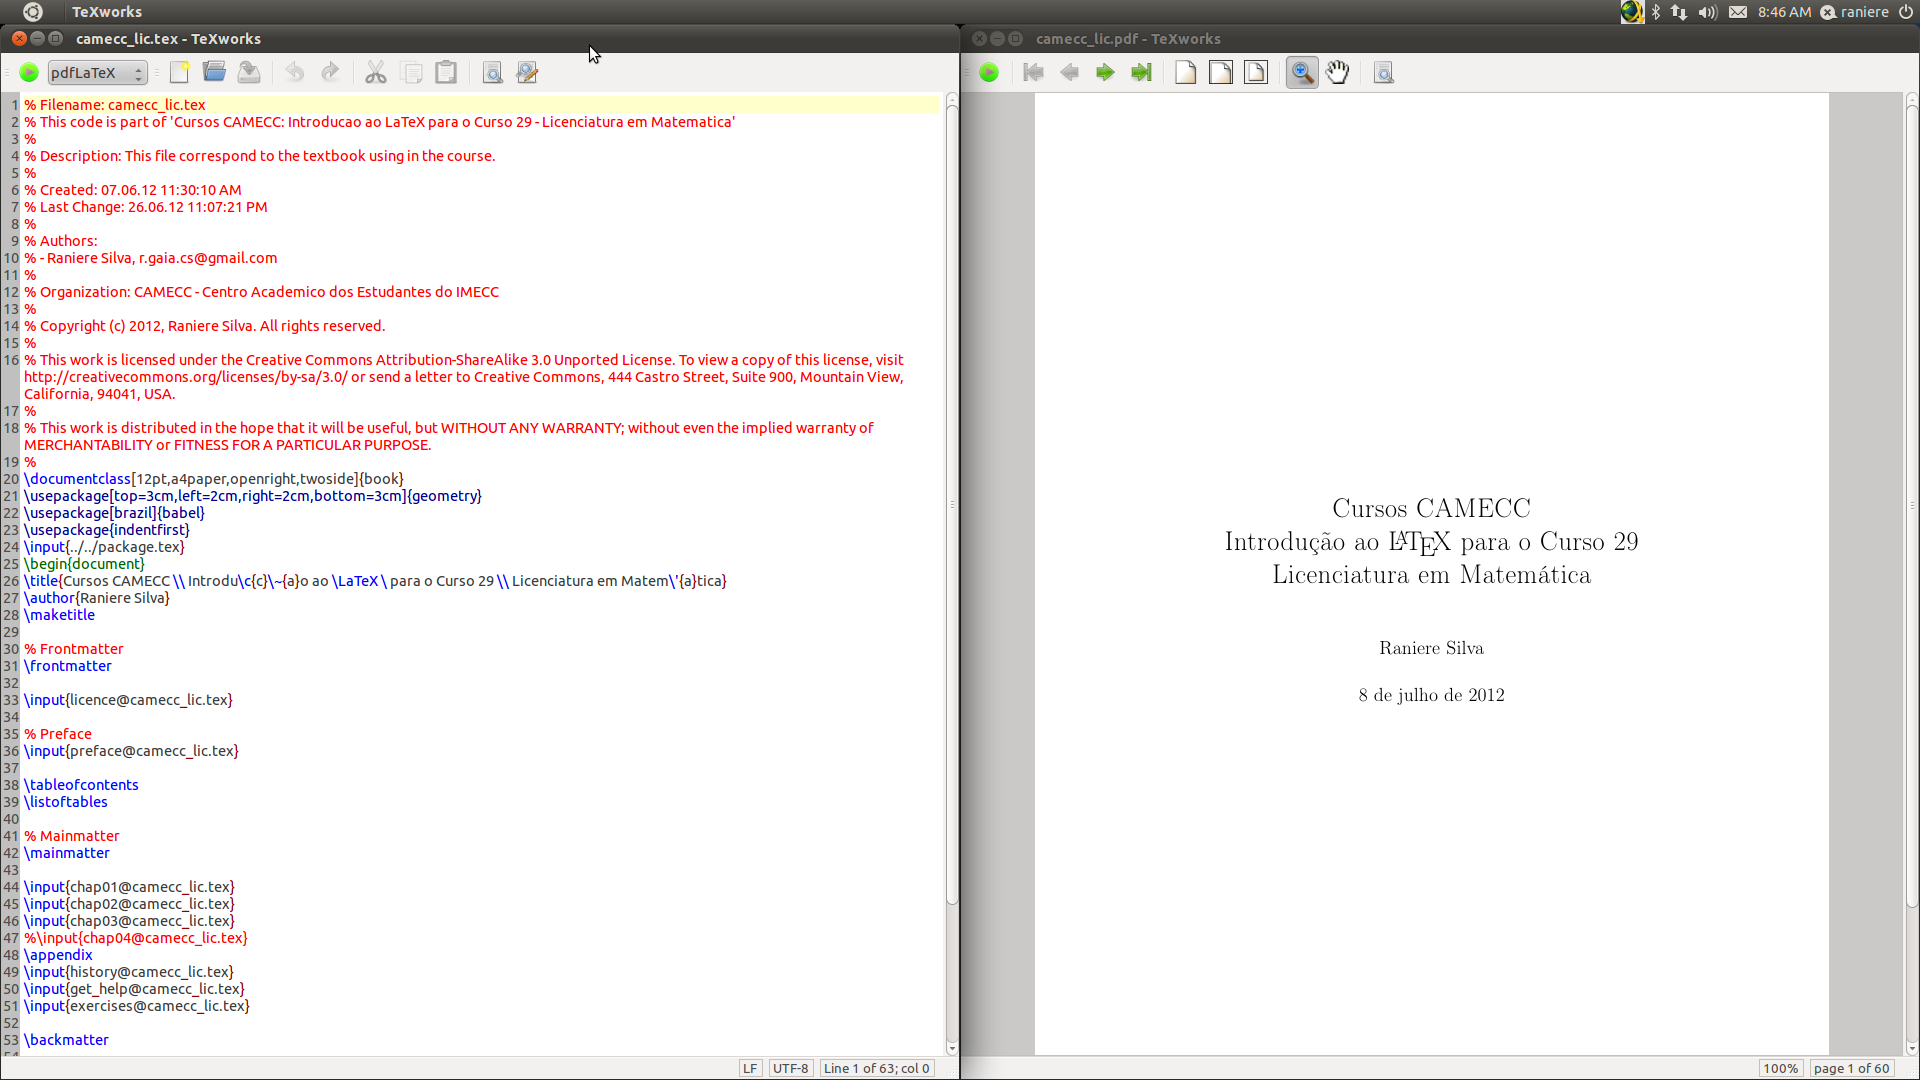
\includegraphics[width=0.4\textwidth]{../../figures/texworks.png} &
        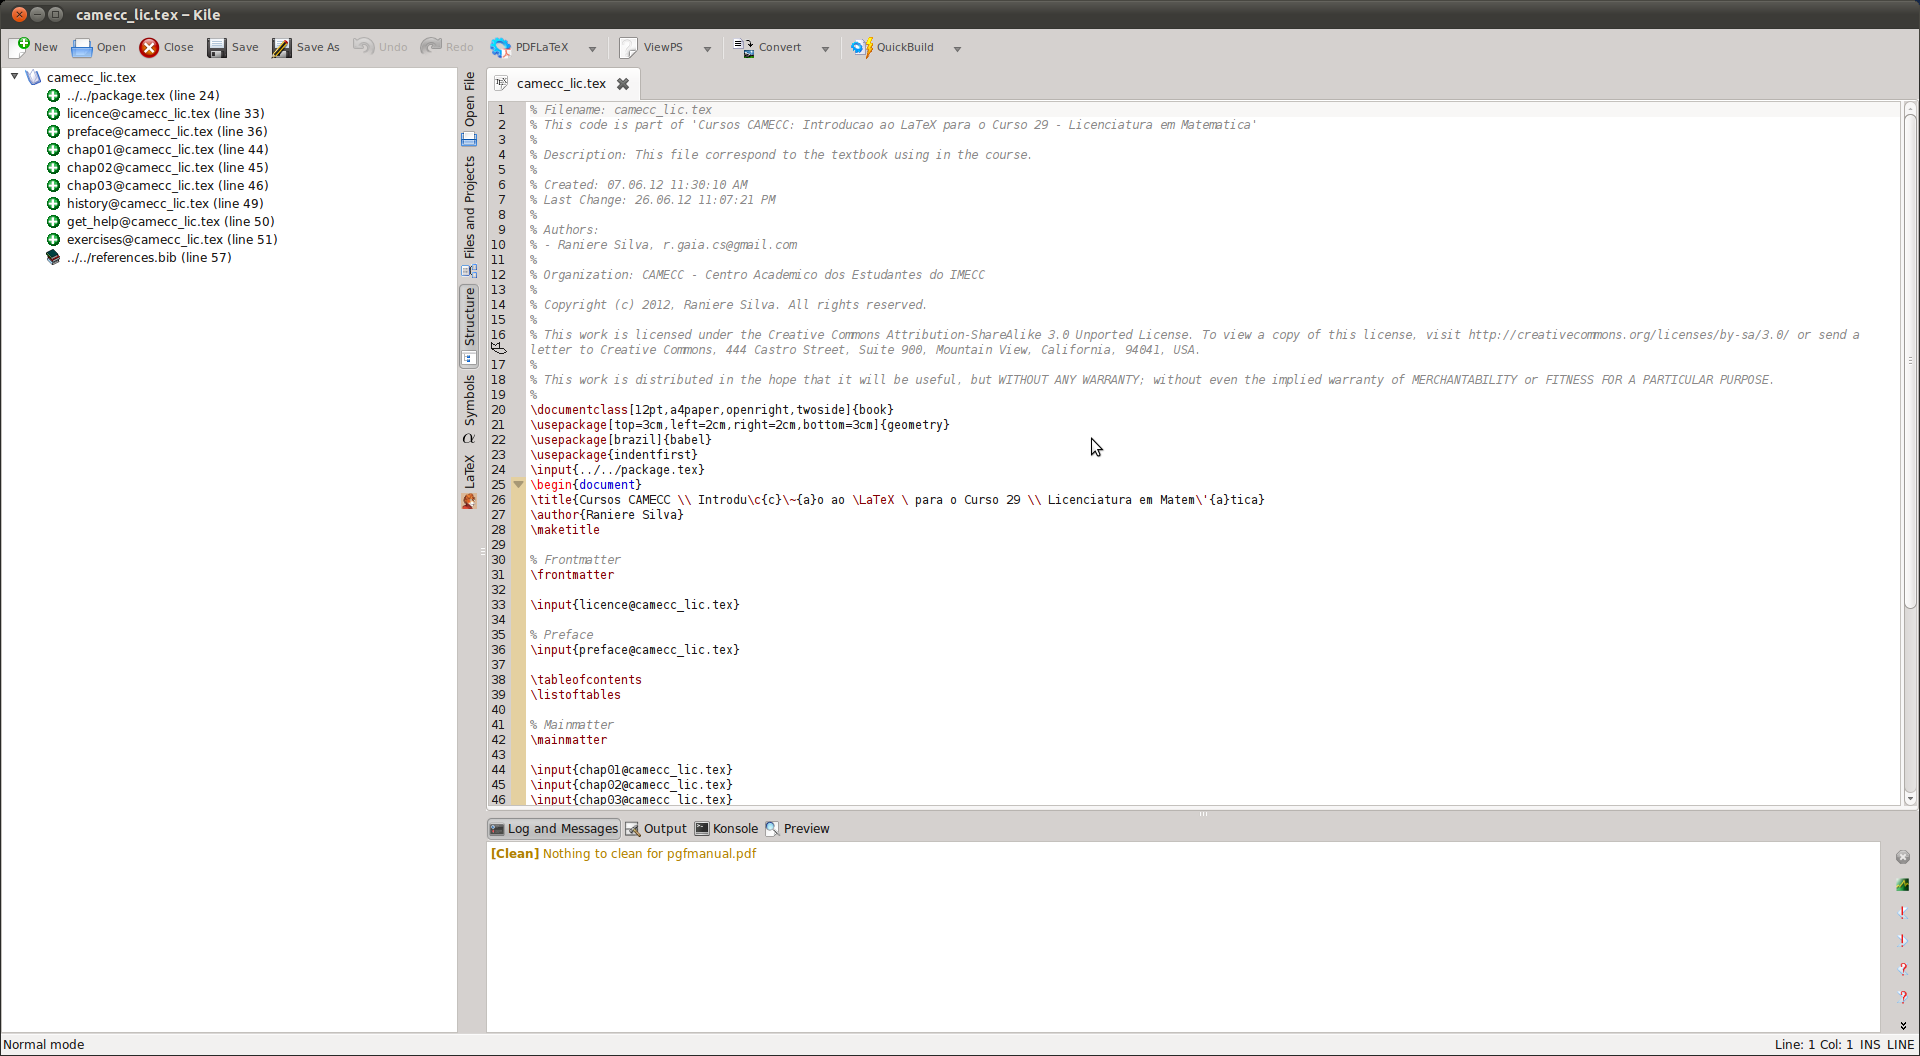
\includegraphics[width=0.4\textwidth]{../../figures/kile.png} \\
        Texworks & Kile \\
        % 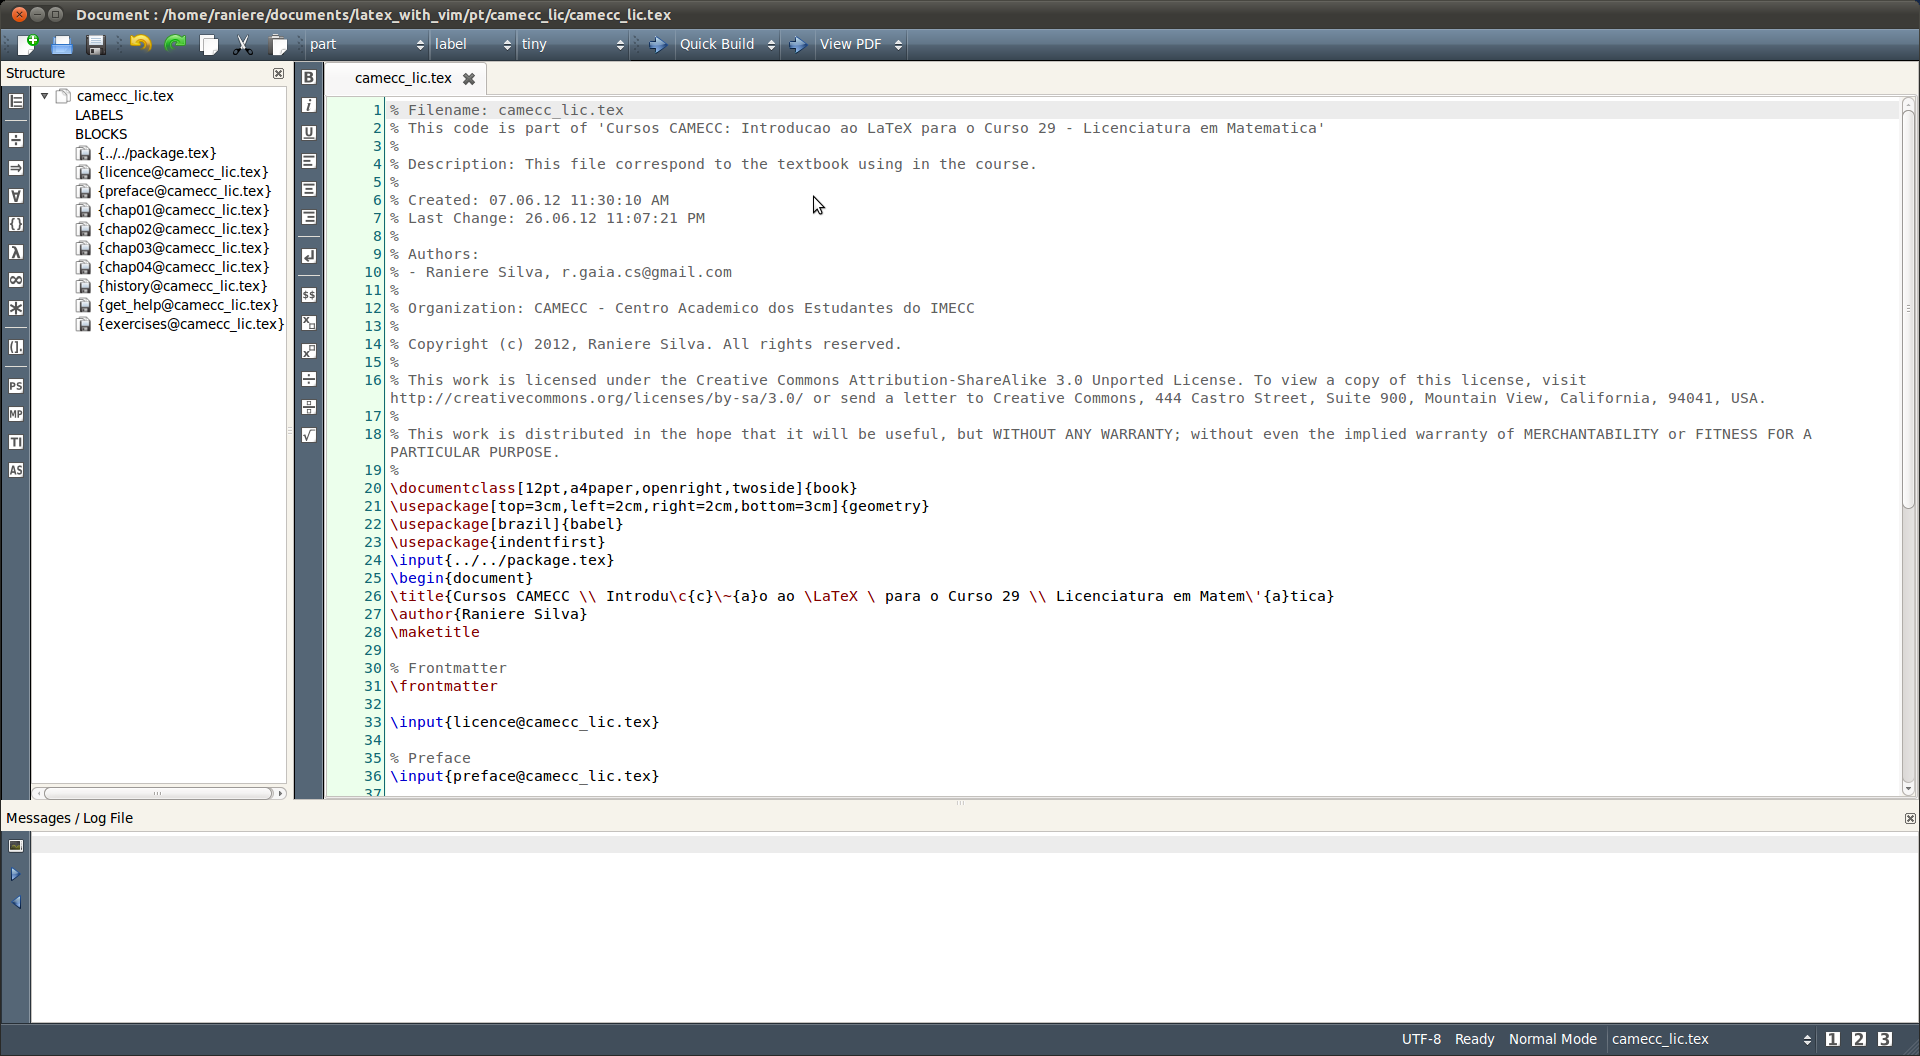
\includegraphics[width=0.4\textwidth]{../../figures/texmaker.png} &
        % 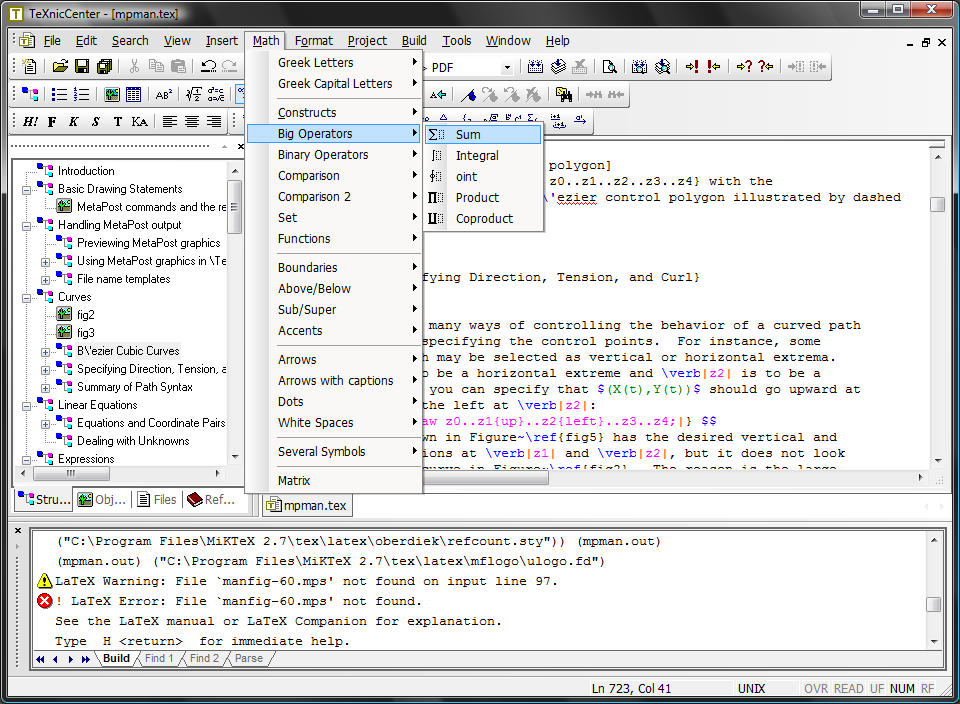
\includegraphics[width=0.4\textwidth]{../../figures/texniccenter.png} \\
        % Texmaker & TexnicCenter \\
        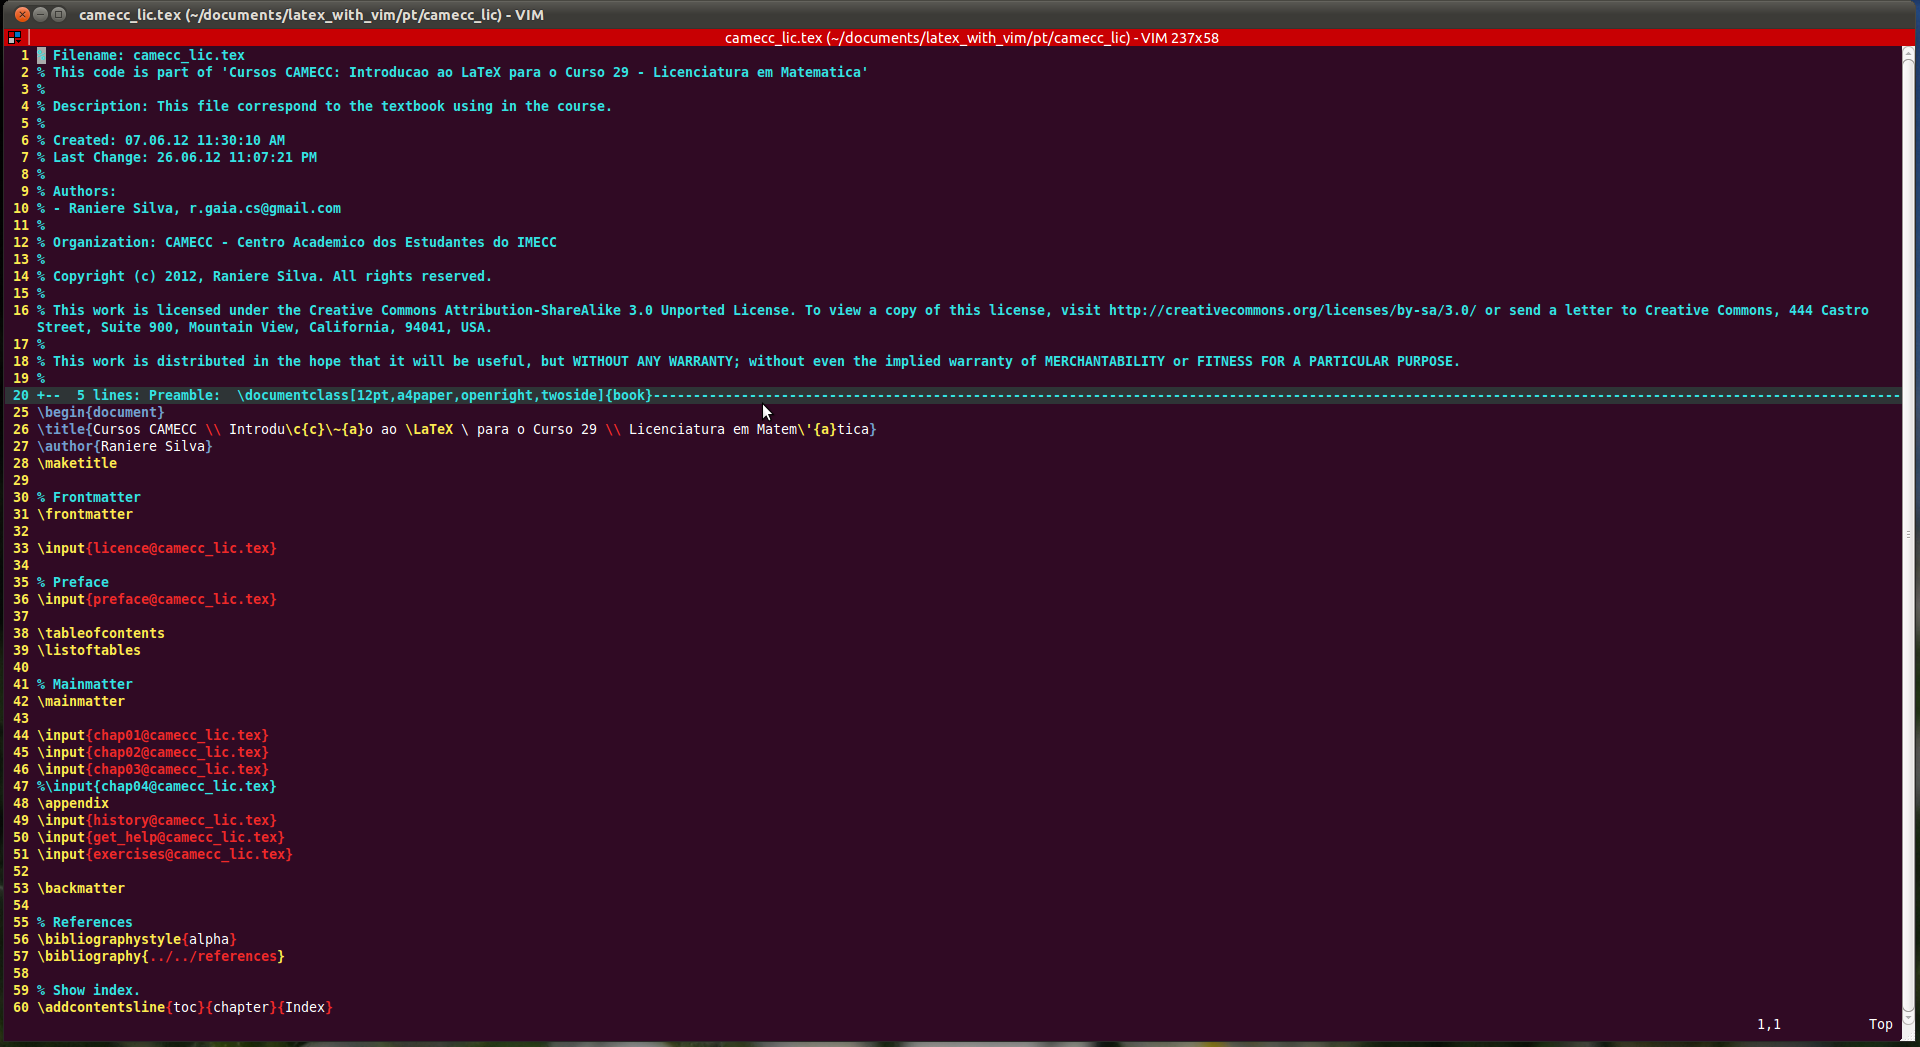
\includegraphics[width=0.4\textwidth]{../../figures/vim.png} &
        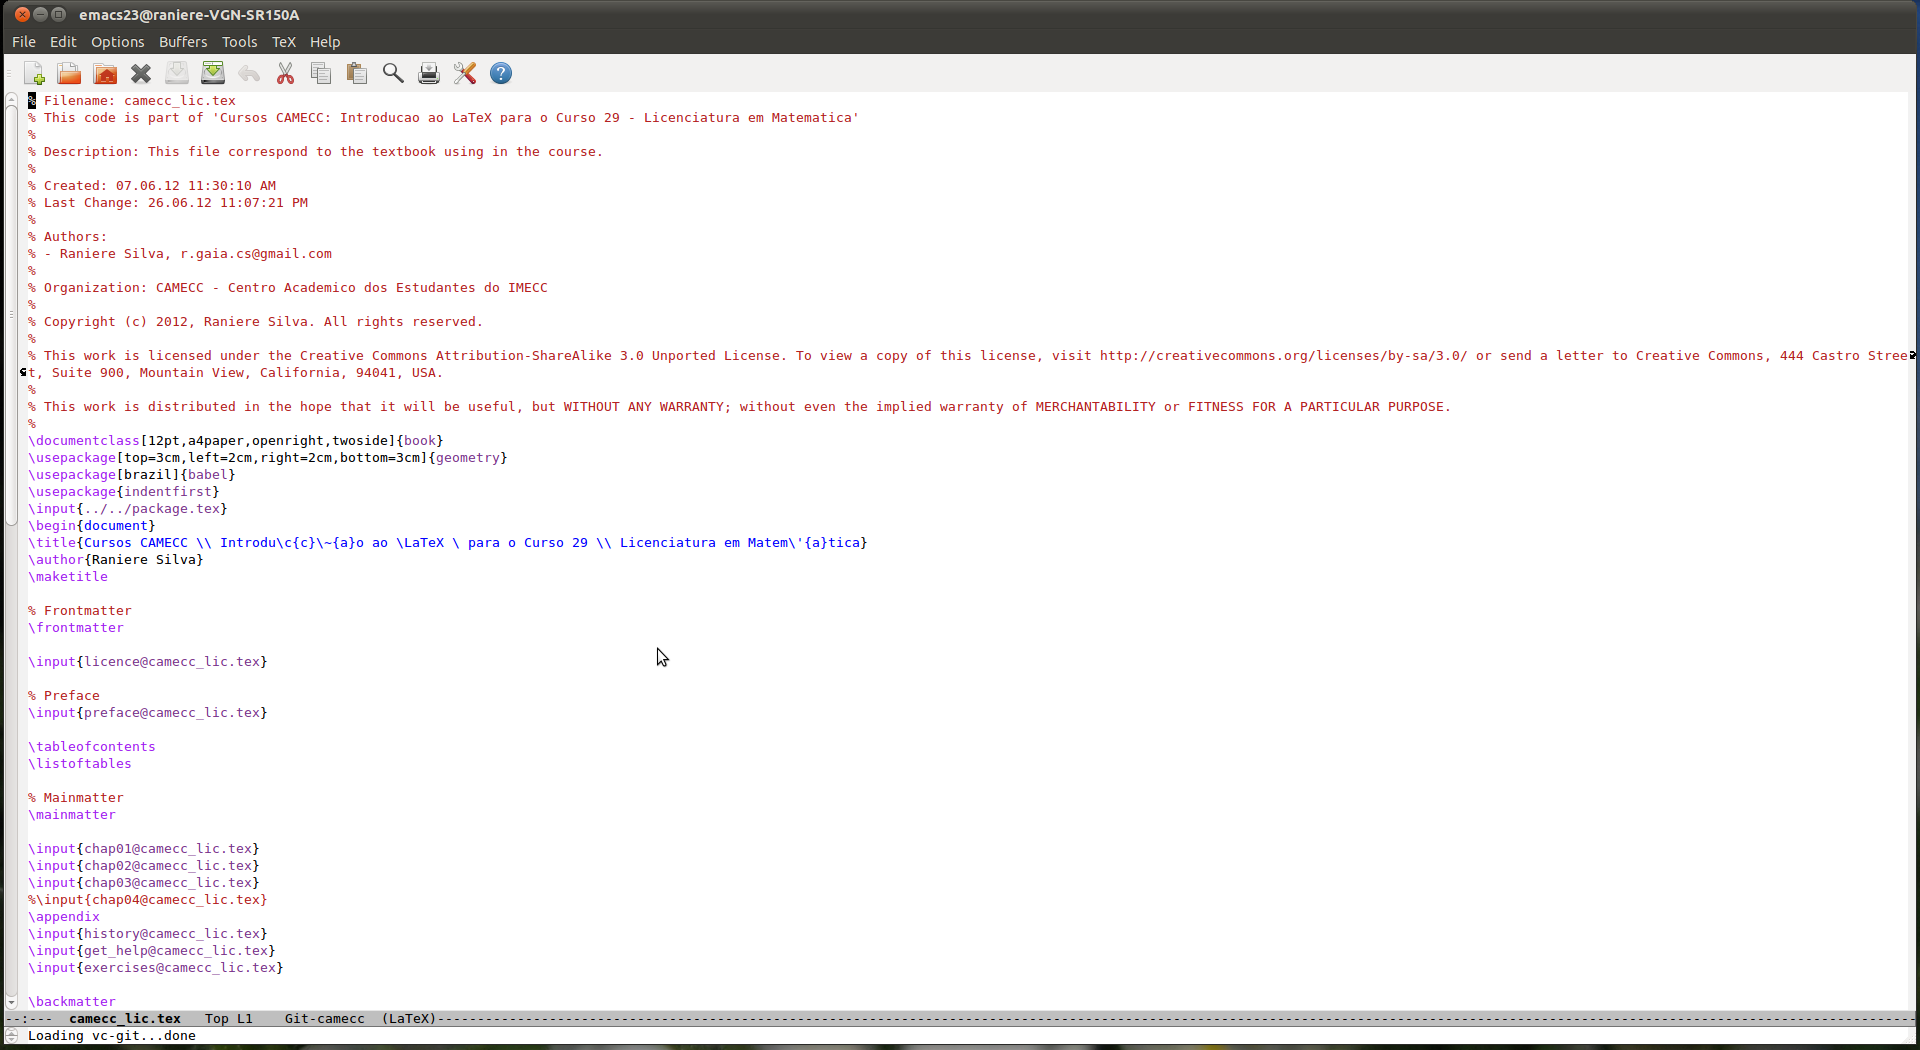
\includegraphics[width=0.4\textwidth]{../../figures/gnu_emacs.png} \\
        Vim & GNU Emacs
    \end{tabular}
    \caption{\flang{Screenshots} de alguns IDE's}
    \label{fig:ide_screenshot}
\end{figure}

\section{Arquivo \lcode{.tex}} \label{sse:basic:tex}
O LaTeX utiliza \lcode{.tex}\index{.tex@\lcode{.tex}} como extensão padrão. O arquivo \lcode{main.tex}, onde \lcode{main} representa o nome do arquivo \lcode{.tex}, é um arquivo de texto, estruturado em duas partes:
\begin{enumerate}
    \item \emph{preâmbulo}\index{preambulo@\emph{pre\^{a}mbulo}}
    \item \emph{informação}\index{informacao@\emph{informa\c{c}\~{a}o}}
\end{enumerate}
sendo que a segunda parte deve ser delimitada pelo ambiente \envname{document}, i.e., ser incluida no lugar de \lcode{XXX} do código abaixo:
\begin{code}
\begin{document}
XXX
\end{document}
\end{code}

\'{E} permito incluir um ou mais arquivo dentro de \lcode{main.tex}, isto é, trabalhar com múltiplos arquivos\index{multiplos arquivos@m\'{u}ltiplos arquivos}. Os arquivos a serem incluídos também possuem a extensão \lcode{.tex} mas devem conter apenas a \emph{informação}.\footnote{Ao trabalhar com múltiplos arquivos apenas precisa-se compilar o arquivo \lcode{main.tex}.}

Uma das forma de incluir um arquivo é com o comando \lstinline!\input!\index{comando!input@\lstinline+\input+}, como ilustrado a seguir:
\begin{code}
\input{aux.tex}
\end{code}
onde \lcode{aux.tex} é o nome do arquivo a ser incluído.\footnote{Caso a extens\~{a}o do arquivo seja suprimida ser\'{a} utilizada \lcode{.tex}.}

Quando \lcode{main.tex} for compilado o arquivo \lcode{aux.tex} será lido e processado exatamente como se tive-se sido inserido na posição que o comando \lstinline!\input! ocupa.

\section{\emph{Preâmbulo}} \label{sse:basic:preamble}
O \emph{preâmbulo}\index{preambulo@\emph{pre\^{a}mbulo}} deve ser iniciado por
\begin{code}
\documentclass[options]{class}
\end{code}
onde \lcode{class}\index{comando!documentclass@\lstinline+\documentclass+} indica o tipo de documento a ser criado e \lcode{options} \'{e} uma lista de palavras chaves separadas por v\'{i}rgula que personaliza o compartamento de \lcode{class} (na Tabela \ref{tab:par_options} encontra-se algumas das palavras chaves disponíveis).
\begin{table}[h!tb]
    \centering
    \caption{Parâmetros disponíveis para \lcode{options}.} \label{tab:par_options}
    \begin{tabular}{llp{0.6\textwidth}}
    \hline
    Função & Código & Descrição \\ \hline
    \multirow{4}{*}{Tamanho} &  & Utiliza, por padrão, o tamanho 10. \\
    & \lcode{10pt} & Tamanho 10. \\
    & \lcode{11pt} & Tamanho 11. \\
    & \lcode{12pt} & Tamanho 12. \\ \hline
    \multirow{7}{*}{Papel} & & Utiliza, por padrão, o tamanho da folha correspondente carta. \\
    & \lcode{letterpaper} & Tamanho da folha correspondente carta. \\
    & \lcode{a4paper} & Tamanho da folha correspondente a A4. \\
    & \lcode{a5paper} & Tamanho da folha correspondente a A5. \\
    & \lcode{b5paper} & Tamanho da folha correspondente a B5. \\
    & \lcode{executivepaper} & Tamanho da folha correspondente a folha executiva. \\
    & \lcode{legalpaper} & Tamanho da folha correspondente a folha legal. \\ \hline
    \multirow{2}{*}{Al. equação} & & Por padrão centra as equações. \\
    & \lcode{fleqn} & Alinha as equações à esquerda. \\ \hline
    \multirow{2}{*}{Nº equação} & & Por padrão enumera as equações à direita. \\
    & \lcode{leqno} & Enumera as equações à esquerda. \\ \hline
    \multirow{4}{*}{Título} & & Por padrão a classe \lcode{article} não começa uma nova página após o título, enquanto que \lcode{report} e \lcode{book} o fazem. \\
    & \lcode{titlepage} & Começa uma nova página após o título. \\
    & \lcode{leqno} & Não começa uma nova página após o título. \\ \hline
    \multirow{4}{*}{Faces} & & Por padrão a classe \lcode{article} e \lcode{report} são a uma face e a classe \lcode{book} é a duas. \\
    & \lcode{oneside} & Gera o documento a uma face. \\
    & \lcode{twoside} & Gera o documento a duas fazes. \\ \hline
    \multirow{5}{*}{Começo} & & Não funciona com a classe \lcode{article} por nesta não existirem capítulos e por padrão a classe \lcode{report} começa os capítulos na próxima página disponível e a classe \lcode{book} sempre nas páginas à direita. \\
    & \lcode{openright} & Começa os capítulos sempre nas páginas à direita. \\
    & \lcode{openany} & Começa os capítulos na próxima página disponível. \\ \hline
    Colunas & \lcode{twocolumn} & Gera o arquivo utilizando-se de duas colunas. \\
    \hline
\end{tabular}

\end{table}

\lcode{class}\index{comando!documentclass@\lstinline+\documentclass+!class@\lcode{class}} corresponde ao nome de um arquivo \lcode{.cls}, os principais são apresentados na Tabela \ref{tab:documentclass} e outros são indicados em \url{http://aprendolatex.wordpress.com/2007/07/15/mais-classes-de-documentos/}. Existe ainda alguns arquivos \lcode{.cls} personalizados disponíveis na internet, destacando-se o \lcode{abnt.cls}, disponível em \url{http://abntex.codigolivre.org.br/}, indicado para documentos que devem seguir as normas da ABNT e o usu\'{a}rio tamb\'{e}m pode escrever sua pr\'{o}pria \lcode{class}.
\begin{table}[h!tb]
    \centering
    \caption{Parâmetros disponíveis para \lcode{class}.} \label{tab:documentclass}
    % Filename: documentclass@latex_with_vim.tex
% This code is part of LaTeX with Vim.
% 
% Description: LaTeX with Vim is free book about Vim, LaTeX and Git.
% 
% Created: 30.03.12 12:12:55 AM
% Last Change: 30.03.12 12:13:08 AM
% 
% Author: Raniere Gaia Costa da Silva, r.gaia.cs@gmail.com
% Organization:  
% 
% Copyright (c) 2010, 2011, 2012, Raniere Gaia Costa da Silva. All rights 
% reserved.
% 
% This file is license under the terms of a Creative Commons Attribution 
% 3.0 Unported License, or (at your option) any later version. More details
% at <http://creativecommons.org/licenses/by/3.0/>.
\begin{tabular}{lp{0.8\textwidth}}
    \hline
    Código & Descrição \\ \hline
    \lcode{article} & Para artigos em revistas especializadas, palestras, trabalhos de disciplinas \dots \\
    \lcode{report} & Para informes maiores que constam de mais de um capítulo, projetos de fim de curso, dissertações, teses e similares. \\
    \lcode{book} & Para livros. \\
    \lcode{slide} & Para transparências. \\
    \lcode{beamer} & Para apresenta\c{c}\~{o}es. \\
    \lcode{exam} & Para lista de exerc\'{i}cios. \\
    \hline
\end{tabular}

\end{table}

O \emph{preâmbulo}\index{preambulo@\emph{pre\^{a}mbulo}} é completado com a inclus\~{a}o de pacotes que serão utilizados na \emph{informação}. O comando para inclus\~{a}o de um pacote\index{comando!usepackage@\lstinline+\usepackage+} segue a seguinte sintaxe:
\begin{code}
\usepackage[options]{package}
\end{code}
onde \lcode{package} é o nome do pacote e \lcode{options} é uma lista de palavras chaves correspondente a op\c{c}\~{o}es do pacote.

Por \'{u}ltimo, \'{e} no \emph{pre\^{a}mbulo} que o usu\'{a}rio tamb\'{e}m pode definir seus pr\'{o}prios comandos e ambientes\footnote{N\~{a}o ser\'{a} abordado neste curso, uma \'{o}tima fonte \'{e} \url{http://en.wikibooks.org/wiki/LaTeX/Customizing_LaTeX}}.

\section{Hello world} \label{sse:basic:hello_world}
Anterioremente foi apresentado os aplicativos necessários para trabalhar com LaTeX e as duas partes principais do arquivo \lcode{.tex}. A seguir apresentaremos como construir a \emph{informação}\index{informacao@\emph{informa\c{c}\~{a}o}}.

O documento mais simples que podemos criar \'{e} apresentado abaixo. \\ 
\begin{minipage}[t]{0.5\linewidth}
    \vspace{-8pt}
    \begin{code}
\documentclass[10pt,a4paper]{article}
\begin{document}
Hello world.
\end{document}
    \end{code}
\end{minipage} \quad \vrule \quad
\begin{minipage}[t]{0.35\linewidth} \vspace{0pt}
    Hello world.
\end{minipage}

Os exemplos que serão apresentados aparecerão seguindo o modelo acima, isto é, em duas colunas sendo a coluna da esquerda contendo o código LaTeX e a coluna da direita contendo a saída obtida. Por simplicidade, nos demais exemplos iremos apresentar apenas a \emph{informação}.

\subsection{Teclado e Idioma}
Na \'{e}poca que o TeX foi desenvolvido utilizava-se a codifica\c{c}\~{a}o ASCII (American Standard Code for Information Interchange) e, consequentemente, o LaTeX foi desenvolvido para utilizar apenas os caracteres presentes na codifica\c{c}\~{a}o ASCII.

As 52 letras (26 letras minúsculas + 26 letras maiúsculas) do alfabeto americano, os dez dígitos indo-arábicos, seis sinais de pontuação (\lstinline+, ; . ? ! :+) e quatro parenteses (\lstinline!( ) [ ]!). Todos estas teclas são interpretadas como elas mesmas pelo LaTeX.

Na seção \ref{sss:basic:space} abordaremos como o LaTeX interpreta o espaço e enter (mudança de linha).

As teclas correspondentes a \lstinline!`!, acento grave, \lstinline!'!, apóstrofe, e \lstinline!-!, hífen, são interpretadas pelo LaTeX de acordo com os caracteres adjacentes.

Os seis símbolos matemáticos (\lstinline!* + = < > /!) são interpretados de maneira diferentes quando no modo texto e no modo matemático\footnote{O modo matemático é apresentado no capítulo \ref{sch:math}.}.

Existem, também, 13 símbolos especiais (\lstinline!# $ % & ~ _ ^ \ { } @ " |!) que são interpretados pelo LaTeX de acordo com os caracteres adjacentes.

Os demais caracteres disponíveis no teclado, quando utilizados, costumam produzir erro.

Para facilitar o uso do LaTeX em outros idiomas que n\~{a}o o ingl\^{e}s pode-se utilizar alguma codificação diferente da ASCII para o arquivo \lcode{.tex}. As codificações mais comuns são UFT-8 e Latin1 sendo que para arquivos codificados com UFT-8 deve-se adicionar a seguinte linha no preâmbulo
\begin{code}
\usepackage[utf8]{inputenc}
\end{code}\index{pacote!inputenc@\pkgname{inputenc}}
enquanto que para arquivos codificados com Latin1
\begin{code}
\usepackage[latin1]{inputenc}
\end{code}
Recomenda-se utilizar a codifica\c{c}\~{a}o UFT-8 (Unicode) pois a Latin1 n\~{a}o possue mais suporte desde 2004 (ver \url{http://pt.wikipedia.org/wiki/ISO_8859-1}) ou apenas os caracteres definidos na codifica\c{c}\~{a}o ASCII pois estes possuem a mesma representa\c{c}\~{a}o na maioria das codifica\c{c}\~{o}es existentes.

É importante que o editor que esteja sendo usado também esteja configurado para trabalhar com a codificação especificada. Quando uma codificação errada estiver sendo usada, o editor pode trocar ou omitir alguns caracteres.

Ao gerar um arquivo pdf utilizando o LaTeX ocorre que copiar e colar um fragmento de texto no pdf com caracteres que n\~{a}o esteja presentes na codifica\c{c}\~{a}o ASCII ser\'{a} preciso corrigir o fragmento. Para atenuar esse trabalho deve-se utilizar o pacote \envname{fontenc}\index{pacote!fontenc@\envname{fontenc}}.

Al\'{e}m disso, deve-se utilizar o pacote \pkgname{babel}\index{pacote!babel@\pkgname{babel}} de Johannes L. Braams que ajusta algumas macros de acordo com o idioma desejado, como a traduções de alguns termos e uso de caixa alta. O pacote \pkgname{babel} que possue as seguintes opções para o idioma português: \lcode{portuges}, \lcode{portuguese}, \lcode{brazil}, \lcode{brazilian}. Maiores detalhes podem ser encontrados na documenta\c{c}\~{a}o do pacote\cite{Braams:2008:Babel}.

\subsection{Espaços, linhas, parágrafos e páginas} \label{sss:basic:space}
No LaTeX o espaço entre palavras apresenta uma particularidade: ele \'{e} ignorado se houver dois ou mais espaços seguidos, como podemos observar a seguir. \\
\example{codes/hello_spaces@latex_with_vim.tex}

Quando for necessário gerar dois ou mais espaços seguidos deve-se utilizar a barra invertida entre os espaços como ilustrado a seguir. \\
\example{codes/hello_spaces_backslash@latex_with_vim.tex}

Nos dois exemplos anteriores é possível verificar que a mudança de linha no código não produz uma nova linha\index{nova linha} no documento gerado. A mudança de linha no LaTeX é representada por \lstinline!\\!\index{comando! @\lstinline+\\+} ou pelo comandos \lstinline!\newline!\index{comando!newline@\lstinline+\newline+}, como ilustrada a seguir. \\
\example{codes/hello_newlines@latex_with_vim.tex}

Já a mudança de parágrafo\index{paragrafo@par\'{a}grafo} é indicada por uma linha em branco. 

Quando for necessário forçar uma mudança de página utiliza-se o comando \lstinline!\newpage!\index{comando!newpage@\lstinline+\newpage+}. Assim como o LaTeX ignora dois ou mais espaços seguidos a mudança de linha e de página também é ignorada.

Por último é importante avisar que, por padr\~{a}o, o primeiro parágrafo de  capítulo, seções, \dots, não é identado. Quando desejar-se identar o primeiro parágrago uma solução é utilizar o pacote \pkgname{indentfirst}.

\subsection{Hifenização}
O LaTeX tenta balancear o tamanho das linhas a serem geradas e para isso utiliza-se de um banco de dados para hifenizar, quando necessário, alguma palavra.

Algumas vezes a hifenização\index{hifenizacao@hifeniza\c{c}\~{a}o} ocorre de maneira inadequada e para corrigir devemos utilizar o comando \lstinline!\hyphenation!\index{comando!hyphenation@\lstinline+\hyphenation+} cujo parâmetro é uma lista de palavras, separadas por espaço, onde o comando - é utilizado para indicar onde a palavra pode ser separada.

\subsection{Acentos}
Embora seja possivel utilizar algumas codifica\c{c}\~{o}es de arquivo que suportam acentua\c{c}\~{a}o utilizando o pacote \pkgname{inputenc} \'{e} importante saber como inserir os acentos utilizando apenas a tabela ASCII que \'{e} apresentado na Tabela~\ref{tab:diacritic}.
\begin{table}[!htb]
    \centering
    \caption{Acentuação (utilizando a vogal ``o'' para exemplo).} \label{tab:diacritic}
    % Filename: diacrict@latex_with_vim.tex
% This code is part of LaTeX with Vim.
% 
% Description: LaTeX with Vim is free book about Vim, LaTeX and Git.
% 
% Created: 30.03.12 12:12:36 AM
% Last Change: 30.03.12 12:12:40 AM
% 
% Author: Raniere Gaia Costa da Silva, r.gaia.cs@gmail.com
% Organization:  
% 
% Copyright (c) 2010, 2011, 2012, Raniere Gaia Costa da Silva. All rights 
% reserved.
% 
% This file is license under the terms of a Creative Commons Attribution 
% 3.0 Unported License, or (at your option) any later version. More details
% at <http://creativecommons.org/licenses/by/3.0/>.
\begin{tabular}{cc|cc|cc|cc}
    \hline
    Comando & Resultado & Comando & Resultado & Comando & Resultado & Comando & Resultado \\ \hline
    \textbackslash '\{o\} & \'{o} & \textbackslash =\{o\} & \={o} & \textbackslash u\{o\} & \u{o} & \textbackslash .\{o\} & \.{o} \\
    \textbackslash v\{o\} & \v{o} & \textbackslash r\{o\} & \r{o} & \textbackslash c\{c\} & \c{c} & \textbackslash t\{oo\} & \t{oo} \\
    \textbackslash \textasciicircum \{o\} & \^{o} & \textbackslash \textasciitilde \{o\} & \~{o} & \textbackslash "\{o\} & \"{o} & \textbackslash d\{o\} & \d{o} \\
    \textbackslash H\{o\} & \H{o} & \textbackslash b\{o\} & \b{o} & \textbackslash `\{o\} & \`{o} & \textbackslash i & \i \\ \hline
\end{tabular}

\end{table}

\section{Caracteres especiais}
No LaTeX alguns caracteres apresentam forma própria de representação. A seguir enunciaremos alguns.

\subsection{Aspas}
Para as aspas\index{aspas} não deve-se usar o caracter de aspas. Para abrir as aspas deve-se utilizar o acento simples e para fechar a aspa simples. \\
\example{codes/quotation_mark@latex_with_vim.tex}

\subsection{Traço}
LaTeX admite três tipos de traço\index{traco@tra\c{c}o}. \\
\example{codes/dashes@latex_with_vim.tex}

\subsection{Pontos sucessivos}
Utiliza-se o comando \lstinline!\dots! ou \lstinline!\ldots! para pontos sucessivos. \\
\example{codes/dots@latex_with_vim.tex}

\subsection{Pontuação e demais símbolos}
Para pontuação\index{pontuacao@pontua\c{c}\~{a}o} e demais símbolos especias deve-se proceder como na Tabela~\ref{tab:symbols}.
\begin{table}[h!tb]
    \centering
    \caption{Para pontuação e símbolos especias.}
    \label{tab:symbols}
    % File: symbols@latex-with-vim.tex
% This code is part of LaTeX with Vim.
% 
% Description: LaTeX with Vim is free book about Vim, LaTeX and Git.
% 
% Created: 30.03.12 12:19:38 AM
% Last Change: 30.03.12 12:19:44 AM
% 
% Author: Raniere Gaia Costa da Silva, r.gaia.cs@gmail.com
% Organization:  
% 
% Copyright (c) 2010, 2011, 2012, Raniere Gaia Costa da Silva. All rights 
% reserved.
% 
% This file is license under the terms of a Creative Commons Attribution 
% 3.0 Unported License, or (at your option) any later version. More details
% at <http://creativecommons.org/licenses/by/3.0/>.

\begin{tabular}{cc|cc|cc}
    \hline
    Comando & Resultado & Comando & Resultado & Comando & Resultado \\ \hline
    \textbackslash \& & \& & \textbackslash textasteriskcentered & \textasteriskcentered & \textbackslash textbackslash & \textbackslash \\
    \textbackslash textbar & \textbar & \textbackslash \{ & \{ & \textbackslash \} & \} \\
    \textbackslash texbullet & \textbullet & \textbackslash textasciitilde & \textasciitilde & \textbackslash textasciicircum & \textasciicircum \\
    \textbackslash copyright & \copyright & \textbackslash textregistered & \textregistered & \textbackslash texttrademark & \texttrademark \\
    \textbackslash textperiodcentered & \textperiodcentered & \textbackslash textexclamdown & \textexclamdown & \textbackslash textquestiondown & \textquestiondown \\
    \textbackslash \% & \% & \textbackslash textgreater & \textgreater & \textbackslash textless & \textless  \\
    \textbackslash \# & \# & \textbackslash S & \S & \textbackslash P & \P \\
    \textbackslash \_ & \_ & \textbackslash dag & \dag & \textbackslash ddag & \ddag \\
    \textbackslash pounds & \pounds & \textbackslash textsuperscript\{a\} & \textsuperscript{a} & \textbackslash textcircled\{a\} & \textcircled{a} \\
    \textbackslash textvisiblespace & \textvisiblespace & \textbackslash \$ & \$ & \textbackslash euro & \euro \\ \hline
\end{tabular}

\end{table}

Destaca-se que para que o símbolo \euro \ seja impresso é necessário que o \emph{preâmbulo} contenha a seguinte linha de código
\begin{code}
    \usepackage[official]{eurosym}
\end{code}

\subsection{Comentários}
Também é possível inserir comentários\index{comentarios@coment\'{a}rios} no arquivo \lcode{.tex}, utilizando-se para isso do caractere \lstinline!%!\index{comando! @\lstinline+%+} de forma que todo o texto posterior ao mesmo e na mesma linha é considerado comentário e não é processado.

\section{Margens}
A configura\c{c}\~{a}o de margens\index{margens} no LaTeX pode ser feita nativamente, utilizando o pacote \pkgname{geometry} ou o pacote \pkgname{fancyhdr}. A seguir abordaremos o pacote \pkgname{geometry} e o estilo de p\'{a}gina.

\subsection{\pkgname{geometry}}
O uso deste pacote é bastante simples, precisa-se apenas fazer a chamada do pacote e atribuir valores para os parâmetros disponíveis. A seguir apresentamos um exemplo:
\begin{code}
\usepackage{geometry}
\geometry{parameter = length, ...}
\end{code}
ou
\begin{code}
\usepackage[parameter = length, ...]{geometry}
\end{code}\index{pacote!geometry@\pkgname{geometry}}

Podemos utilizar \lcode{length} em qualquer unidade disponível no LaTeX, mm, cm e outras. Já as opções para \lcode{parameter} mais utilizadas são apresentadas na Tabela~\ref{tab:par_geometry} e ilustradas na Figura~\ref{fig:par_geometry}.
\begin{table}[h!tb]
    \centering
    \caption{Opções disponíveis para \lcode{parameter}, referente ao pacote \lcode{geometry}.}
    \label{tab:par_geometry}
    % File: geometry@latex-with-vim.tex
% This code is part of LaTeX with Vim.
% 
% Description: LaTeX with Vim is free book about Vim, LaTeX and Git.
% 
% Created: 30.03.12 12:19:38 AM
% Last Change: 30.03.12 12:19:44 AM
% 
% Author: Raniere Gaia Costa da Silva, r.gaia.cs@gmail.com
% Organization:  
% 
% Copyright (c) 2010, 2011, 2012, Raniere Gaia Costa da Silva. All rights 
% reserved.
% 
% This file is license under the terms of a Creative Commons Attribution 
% 3.0 Unported License, or (at your option) any later version. More details
% at <http://creativecommons.org/licenses/by/3.0/>.

\begin{tabular}{lp{0.8\textwidth}}
    \hline
    Código & Descrição \\ \hline
    \lcode{paperwidth} & Largura do papel. \\
    \lcode{paperheight} & Altura do papel. \\
    \lcode{textwidth} & Largura da caixa de texto. \\
    \lcode{textheigth} & Altura da caixa de texto. \\
    \lcode{top} & Margem superior. \\
    \lcode{bottom} & Margem inferior. \\
    \lcode{lefth} & Margem esquerda. \\
    \lcode{right} & Margem direita. \\ \hline
\end{tabular}

\end{table}
\begin{figure}[h!]
    \centering
    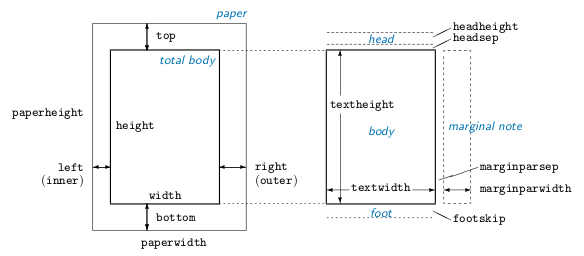
\includegraphics[width=0.8\textwidth]{figures/geometry_margin.png}
    \flushright Fonte: \cite{Umeki:2010:Geometry}
    \caption{Ilustração da opções disponíveis para \lcode{parameter} apresentadas na Tabela \ref{tab:par_geometry}.} \label{fig:par_geometry}
\end{figure}

\subsection{Estilo de p\'{a}gina}

Existe um estilo de página definido como padrão\footnote{Corresponde ao estilo \lcode{plain} apresentado na Tabela \ref{tab:par_style}.}, quando deseja-se mudar o estilo em todo o documento pode-se utilizar o comando
\begin{code}
\pagestyle{style}
\end{code}
e quando for necessário mudá-lo apenas na página atual utiliza-se o comando
\begin{code}
\thispagestyle{style}
\end{code}

As opções para \lcode{style} são apresentadas na Tabela~\ref{tab:par_style}.
\begin{table}[!htb]
    \centering
    \caption{Opções disponíveis para \lcode{style}.}
    \label{tab:par_style}
    % File: style@latex-with-vim.tex
% This code is part of LaTeX with Vim.
% 
% Description: LaTeX with Vim is free book about Vim, LaTeX and Git.
% 
% Created: 30.03.12 12:19:38 AM
% Last Change: 30.03.12 12:19:44 AM
% 
% Author: Raniere Gaia Costa da Silva, r.gaia.cs@gmail.com
% Organization:  
% 
% Copyright (c) 2010, 2011, 2012, Raniere Gaia Costa da Silva. All rights 
% reserved.
% 
% This file is license under the terms of a Creative Commons Attribution 
% 3.0 Unported License, or (at your option) any later version. More details
% at <http://creativecommons.org/licenses/by/3.0/>.

\begin{tabular}{lp{0.8\textwidth}}
    \hline
    Código & Descrição \\ \hline
    \lcode{plain} & Imprime os números de página no centro do pé da página. \\
    \lcode{headings} & No cabeçalho de cada página imprime o capítulo que está sendo processado e o número da página. O pé da página fica vazio. \\
    \lcode{empty} & Coloca tanto o cabeçalho como o pé da página vazios.
\end{tabular}

\end{table}

Aos interessados em criar um estilo próprio, sugere-se utilizar o pacote \lcode{fancyhdr}.
\section{Fonte}
No LaTeX estão disponíveis algumas fontes\index{fonte} opcionais. Comandos da forma \lstinline!\textXX! são responsáveis por alterar a fonte sendo que \lcode{XX} corresponde ao código da fonte a serem utilizados. A Tabela~\ref{tab:text} apresenta alguns das opções disponíveis.
\begin{table}[!htb]
    \centering
    \caption{Opções disponíveis para \lcode{XX} da fonte.} \label{tab:text}
    % Filename: text@latex_with_vim.tex
% This code is part of LaTeX with Vim.
% 
% Description: LaTeX with Vim is free book about Vim, LaTeX and Git.
% 
% Created: 30.03.12 12:19:02 AM
% Last Change: 30.03.12 12:19:06 AM
% 
% Author: Raniere Gaia Costa da Silva, r.gaia.cs@gmail.com
% Organization:  
% 
% Copyright (c) 2010, 2011, 2012, Raniere Gaia Costa da Silva. All rights 
% reserved.
% 
% This file is license under the terms of a Creative Commons Attribution 
% 3.0 Unported License, or (at your option) any later version. More details
% at <http://creativecommons.org/licenses/by/3.0/>.
\begin{tabular}{lp{0.8\textwidth}}
    \hline
    Código & Descrição \\ \hline
    \lcode{it} & Texto em itálico. \\
    \lcode{bf} & Texto em negrito. \\
    \lcode{rm} & Texto em romano. \\
    \lcode{sf} & Texto em sans serif. \\
    \lcode{tt} & Texto na tipografia de uma máquina de escrever. \\
    \lcode{sc} & Texto em caixa alta. \\ \hline
\end{tabular}

\end{table}

A seguir é ilustrado as opções apresentadas na Tabela~\ref{tab:text}. \\
\example{codes/hello_fonte@latex_with_vim.tex}

\subsection{Tamanho}
Uma das maneiras de mudar o tamanho da fonte\index{fonte!tamanho} em uma parte do texto é utilizando um dos ambiente  ou comando de tamanho (a Tabela \ref{tab:op_tamanho_fonte} apresenta algumas opções disponíveis).
\begin{table}[h!tb]
    \centering
    \caption{Opções disponíveis para o tamanho da fonte, em ordem crescente.}
    \label{tab:op_tamanho_fonte}
    % Filename: font_size@latex_with_vim.tex
% This code is part of LaTeX with Vim.
% 
% Description: LaTeX with Vim is free book about Vim, LaTeX and Git.
% 
% Created: 30.03.12 12:12:36 AM
% Last Change: 30.03.12 12:12:40 AM
% 
% Author: Raniere Gaia Costa da Silva, r.gaia.cs@gmail.com
% Organization:  
% 
% Copyright (c) 2010, 2011, 2012, Raniere Gaia Costa da Silva. All rights 
% reserved.
% 
% This file is license under the terms of a Creative Commons Attribution 
% 3.0 Unported License, or (at your option) any later version. More details
% at <http://creativecommons.org/licenses/by/3.0/>.
\begin{tabular}{lp{0.7\textwidth}}
    \hline
    Código & Descrição \\ \hline
    \lstinline!\tiny! & O menor tamanho possível. \\
    \lstinline!\SMALL! ou \lstinline!\scriptsize! &  \\
    \lstinline!\Small! ou \lstinline!\footnotesize! & Tamanho utilizado em notas de rodapé. \\
    \lstinline!\small! &  \\
    \lstinline!\normalsize! & Tamanho padrão. \\
    \lstinline!\large! & \\
    \lstinline!\Large! & \\
    \lstinline!\LARGE! & \\
    \lstinline!\huge! & \\
    \lstinline!\Huge! & O maior tamanho disponível. \\ \hline
\end{tabular}

\end{table}

Destaca-se que os tamanhos são baseados no tamanho padrão. A seguir um exemplo. \\
\example{codes/hello_size@latex_with_vim.tex}

\subsection{Cor}
Para alterar a cor\index{fonte!cor} do texto é necessário os pacotes \pkgname{graphicx}\index{pacote!graphicx@\pkgname{graphicx}} e \pkgname{color}\index{pacote!color@\pkgname{color}} e pode-se utilizar um dos comandos: \lstinline!\textcolor!\index{comando!textcolor@\lstinline+\textcolor+} ou \lstinline!\color!\index{comando!color@\lstinline+\color+}.

A seguir apresentamos um exemplo. \\
\example{codes/hello_color@latex_with_vim.tex}

\subsection{Edição direta}
Algumas vezes deseja-se inserir um texto que não deve ser interpretado. Isso é possível pelo ambiente \envname{verbatim}\index{ambiente!verbatim@\envname{verbatim}}, coloca o texto em uma nova linha, e pelo comando \lstinline!\verb!\index{comando!verb@\lstinline+\verb+}, coloca o texto no mesmo parágrafo.

Tanto o ambiente \lcode{verbatim} como o comando \lstinline!\verb! apresentam uma fonte própria. \\
\example{codes/hello_verb@latex_with_vim.tex}

Vale destacar que o comando \textbackslash\lcode{verb} é ``flexível'' quando ao delimitador, os caracteres \lstinline+!+, \lstinline!+! e \lstinline!:! normalmente exercem satisfatoriamente esta função.

\section{Espaçamento}
Nesta seção abordaremos como inserir espaços\index{espa\c{c}os em branco} ao longo do texto no LaTeX, mas antes é importante destacar que podemos suprimir espaços ao utilizar medidas negativas.

\subsection{Espaçamento horizontal}
Para produzir um espaço horizontal utiliza-se o comando \lstinline!\hspace!\index{comando!hspace@\lstinline+\hspace+} que tem como parâmetro o tamanho do espaço a ser inserido. Se o comando ocorrer entre duas linhas ou no início de uma linha o LaTeX não produz o espaço e para este caso devemos utilizar  \lstinline!\hspace*!.

Para modificar a identação característica de um novo parágrafo deve-se utilizar o comando
\begin{code}
\setlength{\parident}{tam}
\end{code} 
onde \lcode{tam} é o novo tamanho para a identação dos parágrafos. No caso de desejar-se suprimir a identação deve-se utilizar o comando \lstinline!\noindent!.

O comando \lstinline!\hfill! cria um espaço suficiente para dividir o texto de modo que o que estiver antes do comando é alinhado a esquerda e o que estiver depois é alinhado a direita. É permitido utilizar o comando mais de uma vez em uma linha. O comando é ignorado quando ocorrer entre duas linhas ou no início de uma linha, neste caso devemos utilizar \lstinline!\hfill*!.

\subsection{Linha horizontal}
Os comandos \lstinline!\dotfill! e \lstinline!\hrulefill! funcionam de maneira semelhante ao comando \lstinline!\hfill!, mas ao invés de inserir um espaço em branco é introduzido, respectivamente uma linha pontilhada e uma linha contínua.

\subsection{Espaçamento vertical}
No capítulo anterior informamos como mudar de linha, nesta seção vamos trabalhar com o espaço entre as linhas.

O comando \lstinline!\baselineskip[tam]! estabelece o tamanho do espaçamento entre linhas para o texto posterior ao comando. Para modificar o tamanho entre duas linhas específicas pode-se utilizar o comando \lstinline!\\[tam]! inicia uma nova linha de maneira que \lcode{tam} é o espaçamento entre as linhas.

Para aumentar o espaço entre parágrafos pode-se utilizar um dos comandos \lstinline!\smallskip!, \lstinline!\medskip! ou \lstinline!\bigskip!, sendo que o tamanho do espaço está relacionado com o tamanho da fonte padrão do documento.

Os comandos \lstinline!\vspace!\index{comando!vspace@\lstinline+\vspace+} e \lstinline!\vfill! funcionam, respectivamente, de modo muito semelhante aos comandos \lstinline!\hspace! e \lstinline!\hfill! só que na vertical.

\subsection{Linha verticais}
O comando \lstinline!\vrule! produz uma linha vertical.

\section{Alinhamento}
Por padrão, o alinhamento\index{alinhamento} ocorre com a margem esquerda e para alterá-lo pode-se utilizar um dos seguintes ambientes: \envname{center} (para texto centralizado), \envname{flushleft} (alinhamento a esquerda) e \envname{flushright} (alinhamento a direita). \\
\example{codes/align@latex_with_vim.tex}

Também é permitido utilizar os comandos: \lstinline!\centering! (para texto centralizado), \lstinline!\raggedleft! (alinhamento a esquerda) e \lstinline!\raggedright! (alinhamento a direita).

% Filename: chap02@camecc_lic.tex
% This code is part of 'Cursos CAMECC: Introducao ao LaTeX para o Curso 29 - Licenciatura em Matematica'
% 
% Description: This file correspond to the chapter 01 of the textbook using in the course.
% 
% Created: 07.06.12 11:30:49 AM
% Last Change: 07.06.12 11:30:53 AM
% 
% Authors:
% - Raniere Silva, r.gaia.cs@gmail.com
% 
% Organization: CAMECC - Centro Academico dos Estudantes do IMECC
% 
% Copyright (c) 2012, Raniere Silva. All rights reserved.
% 
% This work is licensed under the Creative Commons Attribution-ShareAlike 3.0 Unported License. To view a copy of this license, visit http://creativecommons.org/licenses/by-sa/3.0/ or send a letter to Creative Commons, 444 Castro Street, Suite 900, Mountain View, California, 94041, USA.
%
% This work is distributed in the hope that it will be useful, but WITHOUT ANY WARRANTY; without even the implied warranty of MERCHANTABILITY or FITNESS FOR A PARTICULAR PURPOSE.
%
\chapter{Aproveitando ao m\'{a}ximo o \LaTeX}
Neste capítulo apresentado ferramentas mais avan\c{c}adas do LaTeX  como listas, refer\^{e}ncias cruzadas, tabelas, figuras, bibliografia e outras.

\section{Endere\c{c}os da internet}
Nos endere\c{c}os da internet \'{e} muito comum a presen\c{c}a de caracteres especiais para o LaTeX. Para inserir um endere\c{c}o da internet facilmente pode-se utilizar o comando \lstinline!\verb!\index{comando!verb@\lstinline+\verb+} que foi apresentado no cap\'{i}tulo anterior ou utilizar o comando \lstinline!\url!\index{comando!url@\lstinline+\url+} dispon\'{i}vel no pacote \pkgname{url}\index{pacote!url@\pkgname{url}}.

\section{Nota de rodapé}
Para produzir notas de rodapé\index{nota de rodape@nota de rodap\'{e}} deve-se utilizar o comando \lstinline!\footnote!\index{comando!footnote@\lstinline+\footnote+} que deve ocorrer imediatamente depois da palavra ou texto a que se refere a nota de rodapé e como parâmetro do comando o texto a ser inserido na nota de rodapé.

\section{Referência cruzada} \label{sse:cross_reference}
Existem dois tipos de referência cruzada\index{referencia cruzada@refer\^{e}ncia cruzada}, a primeira para alguma parte do documento e a segunda para um outro documento. Nesta seção abordaremos o primeiro tipo e o segundo n\~{a}o ser\'{a} tratado neste curso\footnote{Os interessados podem dar uma olhada em \url{ttp://en.wikibooks.org/wiki/LaTeX/Bibliography_Management}}.

Para alguns comandos e ambientes o LaTeX atribui um número, ou conjunto de caracteres, que pode ser vinculado a um nome pelo comando \lstinline!\label!\index{comando!label@\lstinline+\label+} e referenciado pelo comando \lstinline!\ref!\index{comando!ref@\lstinline+\ref+} e \lstinline!\pageref!, este \'{u}ltimo quando deseja-se o n\'{u}mero da página onde encontra-se o item referenciado.

O argumento do comando \lstinline!\label! é uma sequencia de caracteres\footnote{Recomenda-se escolher uma sequencia ``amigável''.}, \flang{case sensitive}, que será utilizada como argumento do comando \lstinline!\ref! ao efetuar a referência.

Ao utilizar os comandos \lstinline!\ref! ou \lstinline!\pageref! é aconselhavel precedé-los por um \lstinline!~! para evitar uma quebra de linha antes da refer\^{e}ncia.

\section{Listas}
Para a construção de listas\index{lista} podemos utilizar um dos quatro ambientes: \envname{itemize}, \envname{enumerate}, \envname{description}\footnote{N\~{a}o ser\'{a} tratado neste curso} ou \envname{list}\footnote{N\~{a}o ser\'{a} tratado neste curso}. E para a criação de sublistas basta adicionar um dos ambientes dentro de um já existente.

Cada item de uma lista é identificado, no LaTeX, pelo comando \lstinline!\item!\index{comando!item@\lstinline+\item+} que deve preceder o texto.

\subsection{\envname{itemize}}
O ambiente \envname{itemize}\index{ambiente!itemize@\envname{itemize}} utiliza um símbolo para indicar cada item da lista. \\
\example{codes/itemize@latex_with_vim.tex}

\subsection{\envname{enumerate}}
O ambiente \envname{enumerate}\index{ambiente!enumerate@\envname{enumerate}} numera cada um dos itens da lista. \\
\example{codes/enumerate@latex_with_vim.tex}

Ao utilizar o ambiente \envname{enumerate} \'{e} permitido para cada item adicionar um comando \lstinline!\label! e posteriormente fazer refer\^{e}ncia a este pelo comando \lstinline!\ref!.

\section{Figuras}
No LaTeX é possível inserir figuras\index{figura} contidas em um arquivo de imagem ou desenhar uma\footnote{Ver a Se\c{c}\~{a}o~\ref{sse:tikz}}. Também podemos adicionar uma legenda para a figura.

\subsection{Arquivos de imagem}
Para inserir arquivos de imagem é necessário o pacote \pkgname{graphicx}\index{pacote!graphicx@\pkgname{graphicx}}. A imagem a ser inserida pode encontrar-se em um dos seguintes formatos: \lcode{jpg}, \lcode{png}, \lcode{pdf} ou \lcode{eps}\footnote{Este formato requer instalada o TeX Live 2011 ou superior.}.

O comando \lstinline!\includegraphics!\index{comando!includegraphics@\lstinline+\includegraphics+} é o responsável por indicar a figura que será inserida, sendo a figura inserida ao longo do texto. A síntaxe deste comando é
\begin{code}
\includegraphics[parameter=length]{file}
\end{code}
em que \lcode{parameter} é um comando disponíveis (algumas opções disponíveis são apresentadas na Tabela \ref{tab:figure_size}), \lcode{length} é uma medida para \lcode{parameter} e \lcode{file} é o nome do arquivo que contem a imagem.
\begin{table}[!htb]
    \centering
    \caption{Opções disponíveis para \envname{parameter}.}
    \label{tab:figure_size}
    % Filename: figure_size@latex_with_vim.tex
% This code is part of LaTeX with Vim.
% 
% Description: LaTeX with Vim is free book about Vim, LaTeX and Git.
% 
% Created: 30.03.12 12:13:41 AM
% Last Change: 30.03.12 12:13:48 AM
% 
% Author: Raniere Gaia Costa da Silva, r.gaia.cs@gmail.com
% Organization:  
% 
% Copyright (c) 2010, 2011, 2012, Raniere Gaia Costa da Silva. All rights 
% reserved.
% 
% This file is license under the terms of a Creative Commons Attribution 
% 3.0 Unported License, or (at your option) any later version. More details
% at <http://creativecommons.org/licenses/by/3.0/>.
\begin{tabular}{lp{0.8\textwidth}}
    \hline
    Código & Descrição \\ \hline
    \textsf{width} & Corresponde a largura da figura. \\
    \textsf{height} & Corresponde a altura da figura. \\
    \textsf{scale} & Corresponde a escala da figura. \\
    \textsf{angle} & Corresponde a uma rotação no sentido horário. \\
    \textsf{page} & Apenas para \textsf{PDF}'s, indica a página a ser utilizada. \\ \hline
\end{tabular}

\end{table}

Uma dica é que para \lcode{length} podemos utilizar medidas correspondente a folha escolhida como por exemplo \lstinline!\textwidth! ou \lstinline!\textheight!.\\
\example{codes/includegraphics@latex_with_vim.tex}

Maiores informações podem ser encontradas em \url{http://en.wikibooks.org/wiki/LaTeX/Importing_Graphics}.

\subsection{\envname{figure}}
O ambiente \envname{figure}\index{ambiente!figure@\envname{figure}} possibilita a inclusão de uma legenda para a figura e trabalha a mesma como um objeto flutuante. A síntaxe deste ambiente é
\begin{code}
\begin{figure}[place]
    imagem
    \caption{legend}
    \label{P:imagem}
\end{figure}
\end{code}
onde \lcode{place} é o parâmetro que indica onde a figura deve ser preferencialmente inserida (as opções disponíveis são apresentadas na Tabela \ref{tab:figure_place} e a opção padrão é \lcode{tbp}), \lcode{imagem} corresponde ao código da figura a ser inserida, \lstinline!\caption!\index{comando!caption@\lstinline+\caption+} é o comando correspondente a legenda e \lcode{legend} é o texto a ser apresentado como legenda, \lstinline!\label! é o comando para referência cruzada como já apresentado. \\
\example{codes/figure_centering@latex_with_vim.tex}
\begin{table}[!htb]
    \centering
    \caption{Opções disponíveis para \envname{place}.}
    \label{tab:figure_place}
    % Filename: figure_place@latex_with_vim.tex
% This code is part of LaTeX with Vim.
% 
% Description: LaTeX with Vim is free book about Vim, LaTeX and Git.
% 
% Created: 30.03.12 12:13:22 AM
% Last Change: 30.03.12 12:13:28 AM
% 
% Author: Raniere Gaia Costa da Silva, r.gaia.cs@gmail.com
% Organization:  
% 
% Copyright (c) 2010, 2011, 2012, Raniere Gaia Costa da Silva. All rights 
% reserved.
% 
% This file is license under the terms of a Creative Commons Attribution 
% 3.0 Unported License, or (at your option) any later version. More details
% at <http://creativecommons.org/licenses/by/3.0/>.
\begin{tabular}{lp{0.8\textwidth}}
    \hline
    Código & Descrição \\ \hline
    \textsf{h} & Na posição onde o código se encontra. \\
    \textsf{t} & No topo de uma página. \\
    \textsf{b} & No fim de uma página. \\
    \textsf{p} & Em uma página separada. \\
    \textsf{!} & Modifica algumas configurações a respeito de boa posição para objeto flutuante. \\ \hline
\end{tabular}

\end{table}

Uma dica útil é que o comando \lstinline!\clearpage!\index{comando!clearpage@\lstinline+\clearpage+} que força as figuras pendentes a serem inseridas.

Outras informações podem ser encontradas em \url{http://en.wikibooks.org/wiki/LaTeX/Floats,_Figures_and_Captions}.

\section{Tabelas}
Assim com as figuras, o LaTeX permite construir tabelas\index{tabela} e adicionar legendas \`{a} estas.

\subsection{\envname{tabular}}
O ambiente \envname{tabular}\index{ambiente!tabular@\envname{tabular}} é utilizado para a construção de tabelas no LaTeX e sua síntaxe é
\begin{code}
\begin{tabular}[colunas]
    informacao
\end{tabular}
\end{code}
onde \lcode{colunas} é uma sequência de caracteres, onde cada caractere corresponde a uma coluna e o respectivo alinhamento que são apresentados na Tabela~\ref{tab:par_colunas}, e \lcode{informacao} é o conteudo de cada célula da tabela.
\begin{table}[h!tb]
    \centering
    \caption{Opções disponíveis para \envname{colunas}.}
    \label{tab:par_colunas}
    % Filename: tabular_halign@latex_with_vim.tex
% This code is part of LaTeX with Vim.
% 
% Description: LaTeX with Vim is free book about Vim, LaTeX and Git.
% 
% Created: 30.03.12 12:11:31 AM
% Last Change: 30.03.12 12:11:38 AM
% 
% Author: Raniere Gaia Costa da Silva, r.gaia.cs@gmail.com
% Organization:  
% 
% Copyright (c) 2010, 2011, 2012, Raniere Gaia Costa da Silva. All rights 
% reserved.
% 
% This file is license under the terms of a Creative Commons Attribution 
% 3.0 Unported License, or (at your option) any later version. More details
% at <http://creativecommons.org/licenses/by/3.0/>.
\begin{tabular}{lp{0.8\textwidth}}
    \hline
    Código & Descrição \\ \hline
    \envname{l} & Alinha com margem esquerda. \\
    \envname{r} & Alinha com a margem direita. \\
    \envname{c} & Centralizado. \\
    \envname{p} & Requer como parâmetro a largura da columa. \\
    \textbar & Imprime uma linha separando as colunas. \\ \hline
\end{tabular}

\end{table}

Cada célula da tabela deve ser separadas pelo comando \lstinline!&!\index{comando! @\lstinline+&+} e a mudança de linha ocorre pelo comando \lstinline!\\!\index{comando! @\lstinline+\\+} ou \lstinline!\tabularnewline!\index{comando!tabularnewline@\lstinline+\tabularnewline+}. Para imprimir uma linha horizontal separando duas linhas da tabela deve-se utilizar o comando \lstinline!\hline!.\\
\example{codes/tabular@latex_with_vim.tex}

Outros comandos também são importantes para a construção mas não trataremos deles aqui, para conhec\^{e}-los visitar \url{http://en.wikibooks.org/wiki/LaTeX/Tables}.

\subsection{\envname{table}}
O ambiente \envname{table}\index{ambiente!table@\envname{table}} possibilita a inclusão de uma legenda para a tabela e trabalha a mesma como um objeto flutuante. A síntaxe deste ambiente, muito semelhante com a do ambiente \envname{figure}, é
\begin{code}
\begin{table}[place]
    tabela
    \caption{legend}
    \label{P:tebela}
\end{table}
\end{code}
onde \lcode{place} é o parâmetro que indica onde a tabela deve ser preferencialmente inserida (as opções disponíveis são apresentadas na Tabela \ref{tab:par_place_tab} e a opção padrão é \lcode{tbp}), \lcode{tabela} corresponde ao código da tabela a ser inserida, \lstinline!\caption!\index{comando!caption@\lstinline+\caption+} é o comando correspondente a legenda e \lcode{legend} é o texto a ser apresentado como legenda, \lstinline!\label! é o comando para referência cruzada como já apresentado. \\
\example{codes/table@latex_with_vim.tex}
\begin{table}[!htb]
    \centering
    \caption{Opções disponíveis para \envname{place}.}
    \label{tab:par_place_tab}
    % Filename: table_place@latex_with_vim.tex
% This code is part of LaTeX with Vim.
% 
% Description: LaTeX with Vim is free book about Vim, LaTeX and Git.
% 
% Created: 30.03.12 12:11:31 AM
% Last Change: 30.03.12 12:11:38 AM
% 
% Author: Raniere Gaia Costa da Silva, r.gaia.cs@gmail.com
% Organization:  
% 
% Copyright (c) 2010, 2011, 2012, Raniere Gaia Costa da Silva. All rights 
% reserved.
% 
% This file is license under the terms of a Creative Commons Attribution 
% 3.0 Unported License, or (at your option) any later version. More details
% at <http://creativecommons.org/licenses/by/3.0/>.
\begin{tabular}{lp{0.8\textwidth}}
    \hline
    Código & Descrição \\ \hline
    \envname{h} & Na posição onde o código se encontra. \\
    \envname{t} & No topo de uma página. \\
    \envname{b} & No fim de uma página. \\
    \envname{p} & Em uma página separada. \\
    \envname{!} & Modifica algumas configurações a respeito de boa posição para objeto flutuante. \\ \hline
\end{tabular}

\end{table}

Uma dica útil é que o comando \lstinline!\clearpage!\index{comando!clearpage@\lstinline+\clearpage+} força as tabelas pendentes a serem inseridas.

\subsection{Extens\~{a}o Calc2LaTeX}
Muitas vezes temos uma tabela no Calc\footnote{O Calc é um dos aplicativos do pacote Openoffice e corresponde ao popular Excel do pacote Microsoft Office.} e desejamos transportá-la para o LaTeX. Para essa tarefa a extens\~{a}o/macro Calc2LaTeX, disponível gratuitamente em \url{http://extensions.services.openoffice.org/en/project/Calc2LaTeX}, é bastante eficiente.

\section{Citações}
No LaTeX encontramos dois ambientes dedicados a citações. O primeiro deles é o \envname{quote}\index{ambiente!quote@\envname{quote}} próprío para citações de uma única linha e o segundo é o \envname{quotation}\index{ambiente!quotation@\envname{quotation}} adequado para citações de vários parágrafos.

% Filename: chap03@camecc_lic.tex
% This code is part of 'Cursos CAMECC: Introducao ao LaTeX para o Curso 29 - Licenciatura em Matematica'
% 
% Description: This file correspond to the chapter 01 of the textbook using in the course.
% 
% Created: 07.06.12 11:30:49 AM
% Last Change: 07.06.12 11:30:53 AM
% 
% Authors:
% - Raniere Silva, r.gaia.cs@gmail.com
% 
% Organization: CAMECC - Centro Academico dos Estudantes do IMECC
% 
% Copyright (c) 2012, Raniere Silva. All rights reserved.
% 
% This work is licensed under the Creative Commons Attribution-ShareAlike 3.0 Unported License. To view a copy of this license, visit http://creativecommons.org/licenses/by-sa/3.0/ or send a letter to Creative Commons, 444 Castro Street, Suite 900, Mountain View, California, 94041, USA.
%
% This work is distributed in the hope that it will be useful, but WITHOUT ANY WARRANTY; without even the implied warranty of MERCHANTABILITY or FITNESS FOR A PARTICULAR PURPOSE.
%
\chapter{Matem\'{a}tica no \LaTeX, amsmath} \label{sch:math}
Neste capítulo abordaremos o modo matemático do LaTeX, com uma \^{e}nfase nos pacotes amsmath\index{pacote!amsmath@\pkgname{amsmath}}, amsfonts, amssymb e amsthm.

\section{Modo matemático}
Para que expressões matemáticas seja processadas corretamentes, deve-se mudar do modo texto para o modo matemático, o que pode ser feito de várias maneiras.

A apresentação de expressões matemáticas pode ocorrer de duas maneiras: \flang{inline}\index{modo matematico@modo matem\'{a}tico!inline@\flang{inline}}, quando aparecem na mesma linha do texto, e \flang{displayed}\index{modo matematico@modo matem\'{a}tico!displayed@\flang{displayed}}, quando aparecem em uma linha própria e centralizada (podendo ou n\~{a}o ser numerada\footnote{Deve-se numerar apenas equa\c{c}\~{o}es as quais ser\~{a}o feita refer\^{e}ncias posteriormente.}).

A seguir, informaremos como proceder para produzir expressões matemáticas \flang{inline} ou \flang{displayed}. Ao final, apresentaremos algumas dicas sobre o uso de express\~{o}es \flang{inline} e \flang{displayed}.

\subsection{\flang{Inline}}
Expressões matemáticas \flang{inline}\index{modo matematico@modo matem\'{a}tico!inline@\flang{inline}} devem ser iniciadas por \lstinline!$! e fechadas por \lstinline!$! ou iniciadas por \lstinline!\)! e fechadas por \lstinline!\)!. \\
\example{codes/math_inline@latex_with_vim.tex}

\subsection{\flang{Displayed}}
Expressões matemáticas \flang{displayed}\index{modo matematico@modo matem\'{a}tico!displayed@\flang{displayed}} devem ser iniciadas por \lstinline!$$! e fechadas por \lstinline!$$! ou iniciadas por \lstinline!\[! e fechadas por \lstinline!\]!. \\
\example{codes/math_display@latex_with_vim.tex}

Alguns ambientes, como \envname{equation}, \envname{eqnarray} e \envname{align}, também produzem expressões matemáticas \flang{displayed}.

\subsection{Uso de \flang{inline} e \flang{displayed}}
Um \'{o}timo resumo sobre quando usar express\~{o}es \flang{inline} e \flang{displayed} encontra-se em \url{http://www.math.uiuc.edu/~hildebr/tex/displays.html}\nocite{Hildebrand:TeX_Resoures} e a seguir apresentaremos tradu\c{c}\~{a}o de alguns trechos. Para maiores detalhes recomenda-se uma leitura na obra ``Mathematics Into Type''\nocite{Swanson:1999:Mathematics}.

Express\~{o}es \flang{inline} s\~{a}o ``feias'' quando apresentam fra\c{c}\~{o}es, somat\'{o}rios, integrais, \ldots e algumas vezes precisam de um cuidado especial para respeitarem as margens. Entretanto, deve-se preferir utilizar express\~{o}es \flang{displayed} apenas nas seguintes ocasi\~{o}es:
\begin{itemize}
    \item a express\~{a}o \'{e} longa (ocupa mais da metade de uma linha);
    \item a express\~{a}o requer bastante espa\c{c}o vertical, i.e., possue v\'{a}rias fra\c{c}\~{o}es, somat\'{o}rios, integrais, \ldots;
    \item a equa\c{c}\~{a}o ser\'{a} numerada;
    \item a express\~{a}o que voc\^{e} deseja destacar/enfatizar.
\end{itemize}

\section{Primeiros comandos no modo matemático}
A seguir enunciaremos como proceder para produzir as primeiras equações, mas antes é importante saber que o modo matemático ignora qualquer espaço (para inserir um espa\c{c}o em branco no modo matem\'{a}tico veja a se\c{c}\~{a}o \ref{sss:math:textos_e_espacamentos}).

\subsection{Operações aritméticas básicas}
As operações aritméticas básicas\index{modo matematico@modo matem\'{a}tico!operacoes aritmeticas basicas@opera\c{c}\~{o}es aritm\'{e}ticas b\'{a}sicas} são escritas normalmente, exceto pela multiplicação que utiliza-se dos comandos \lstinline!\times! ou \lstinline!\cdot!\footnote{O uso do comando mais adequado depende muito do campo de estudo.} e das frações representada pelo comando \lstinline!\frac!\footnote{Deve-se ponderar o uso deste comando por quest\~{a}o de legibilidade.}. \\
\example{codes/math_powers_indices@latex_with_vim.tex}

\subsection{Índices e expoentes}
\'{I}ndices\index{modo matematico@modo matem\'{a}tico!indice@\'{i}ndice} e expoentes\index{modo matematico@modo matem\'{a}tico!expoente} são indicados pelos respectivos comandos: \flang{underscore}, \lcode{_}, e \flang{caret}, \lcode{^}. Por padrão apenas o primeiro símbolo depois do comando é alterado, quando for necessário mais de um símbolo deve-se utilizar chaves.

O símbolo \flang{prime}, muito utilizado para derivadas, já vem posicionado corretamente.\footnote{Algumas vezes deve-se preferir utilizar o comando \lcode{prime} em conjunto com \flang{underscore} e/ou \flang{caret}.} \\
\example{codes/math_powers_indices@latex_with_vim.tex}

\subsection{Acentos}
Os acentos\index{modo matematico@modo matem\'{a}tico!acento} disponíveis no modo matemático são apresentados na Tabela~\ref{tab:math_accents}.
\begin{table}[h!tb]
    \centering
    \caption{Acentos disponíveis no modo matemático.}
    \label{tab:math_accents}
    % Filename: math_accents@latex_with_vim.tex
% This code is part of LaTeX with Vim.
% 
% Description: LaTeX with Vim is free book about Vim, LaTeX and Git.
% 
% Created: 30.03.12 12:14:55 AM
% Last Change: 30.03.12 12:15:01 AM
% 
% Author: Raniere Gaia Costa da Silva, r.gaia.cs@gmail.com
% Organization:  
% 
% Copyright (c) 2010, 2011, 2012, Raniere Gaia Costa da Silva. All rights 
% reserved.
% 
% This file is license under the terms of a Creative Commons Attribution 
% 3.0 Unported License, or (at your option) any later version. More details
% at <http://creativecommons.org/licenses/by/3.0/>.
\begin{tabular}{cc|cc|cc}
    \hline
    Comando & Resultado & Comando & Resultado & Comando & Resultado \\ \hline
    \textbackslash\textsf{acute\{a\}} & $\acute{a}$ & \textbackslash\textsf{bar\{a\}} & $\bar{a}$ & \textbackslash\textsf{breve\{a\}} & $\breve{a}$ \\
    \textbackslash\textsf{check\{a\}} & $\check{a}$ & \textbackslash\textsf{dot\{a\}} & $\dot{a}$ & \textbackslash\textsf{ddot\{a\}} & $\ddot{a}$ \\
    \textbackslash\textsf{dddot\{a\}} & $\dddot{a}$ & \textbackslash\textsf{ddddot\{a\}} & $\ddddot{a}$ & \textbackslash\textsf{grave\{a\}} & $\grave{a}$ \\
    \textbackslash\textsf{hat\{a\}} & $\hat{a}$ & \textbackslash\textsf{widehat\{a\}} & $\widehat{a}$ & \textbackslash\textsf{mathring\{a\}} & $\mathring{a}$ \\
    \textbackslash\textsf{tilde\{a\}} & $\tilde{a}$ & \textbackslash\textsf{widetilde\{a\}} & $\widetilde{a}$ & \textbackslash\textsf{vec\{a\}} & $\vec{a}$ \hfill
\end{tabular}

\end{table}

\subsection{Delimitadores}
Parênteses\index{modo matematico@modo matem\'{a}tico!parenteses@par\^{e}nteses|see{delimitadores}}, colchetes\index{modo matematico@modo matem\'{a}tico!colchetes|see{delimitadores}} e chaves\index{modo matematico@modo matem\'{a}tico!chaves|see{delimitadores}} são exemplos de delimitadores\index{modo matematico@modo matem\'{a}tico!delimitadores}. Uma lista completa dos delimitadores dispon\'{i}veis no LaTeX encontra-se na Tabela~\ref{tab:math_delimiter}.
\begin{table}[h!tb]
    \centering
    \caption{Delimitadores disponíveis no LaTeX.}
    \label{tab:math_delimiter}
    % Filename: math_delimiter@latex_with_vim.tex
% This code is part of LaTeX with Vim.
% 
% Description: LaTeX with Vim is free book about Vim, LaTeX and Git.
% 
% Created: 30.03.12 12:16:24 AM
% Last Change: 30.03.12 12:16:29 AM
% 
% Author: Raniere Gaia Costa da Silva, r.gaia.cs@gmail.com
% Organization:  
% 
% Copyright (c) 2010, 2011, 2012, Raniere Gaia Costa da Silva. All rights 
% reserved.
% 
% This file is license under the terms of a Creative Commons Attribution 
% 3.0 Unported License, or (at your option) any later version. More details
% at <http://creativecommons.org/licenses/by/3.0/>.
\begin{tabular}{>{\centering}p{0.13\linewidth}<{\centering}>{\centering}p{0.07\linewidth}<{\centering}|>{\centering}p{0.13\linewidth}<{\centering}>{\centering}p{0.07\linewidth}<{\centering}|>{\centering}p{0.13\linewidth}<{\centering}>{\centering}p{0.07\linewidth}<{\centering}|>{\centering}p{0.13\linewidth}<{\centering}>{\centering}p{0.07\linewidth}<{\centering}}
    \hline
    Com. & Res. & Com. & Res. & Com. & Res. & Com. & Res. \tabularnewline \hline
    \lstinline!(! & $($ & \lstinline!)! & $)$ & \lstinline![! & $[$ & \lstinline!]! & $]$ \tabularnewline
    \lstinline!\{! & $\{$ & \lstinline!\}! & $\}$ & \lstinline!\backslash! & $\backslash$ & \lstinline!/! & $/$ \tabularnewline
    \lstinline!\langle! & $\langle$ & \lstinline!\rangle! & $\rangle$ & \lstinline!|! & $|$ & \lstinline!\|! & $\|$ \tabularnewline
    \lstinline!\lfloor! & $\lfloor$ & \lstinline!\rfloor! & $\rfloor$ & \lstinline!\lceil! & $\lceil$ & \lstinline!\rceil! & $\rceil$ \tabularnewline
    \lstinline!\ulcorner! & $\ulcorner$ & \lstinline!\urcorner! & $\urcorner$ &\lstinline!\llcorner! & $\llcorner$ & \lstinline!\lrcorner! & $\lrcorner$ \tabularnewline \hline
\end{tabular}
\begin{flushleft}
    \textbf{Nota:} Enquanto que \lstinline!|! \'{e} um limitador \lstinline!\mid! \'{e} um operador l\'{o}gico.
\end{flushleft}

\end{table}

Para expressões matemáticas no modo \flang{displayed} ou longas é aconselável utilizar os comandos \lstinline!\left! e \lstinline!\right! anteriormente ao limitador para ajustá-lo verticalmente. \\
\example{codes/math_delimiters_sizes@latex_with_vim.tex}

\subsection{Textos e espa\c{c}amentos} \label{sss:math:textos_e_espacamentos}
Existem tr\^{e}s ocasi\~{o}es em que \'{e} preciso inserir um texto\index{modo matematico@modo matem\'{a}tico!texto} dentro de uma express\~{a}o matem\'{a}tica:
\begin{itemize}
    \item um operador matem\'{a}tico \'{e} representado pelas primeiras letras de seu nome, e.g., $\max$, $\min$, $\lim$, \ldots;
    \item uma vari\'{a}vel \'{e} representada por mais de uma letra;
    \item incluir uma explica\c{c}\~{a}o/justificativa.
\end{itemize}

O LaTeX j\'{a} possue v\'{a}rios operadores matem\'{a}ticos definidos (s\~{a}o apresentados mais a frente) e quando o operador desejado n\~{a}o estiver definido deve-se utilizar o comando \lstinline!\operatorname!\index{modo matematico@modo matem\'{a}tico!novos operadores} ou \lstinline!\DeclareMathOperator!, este \'{u}ltimo quando o operador for ser utilizado v\'{a}rias vezes no documento. 

Em rela\c{c}\~{a}o ao nome de vari\'{a}veis\index{modo matematico@modo matem\'{a}tico!nomes longos para variaveis@nomes longos para vari\'{a}veis}, deve-se evitar ao m\'{a}ximo nome\'{a}-las com mais de uma letra (utilizar o alfabeto grego para isso). Quando n\~{a}o for poss\'{i}vel evitar, deve-se utilizar o comando \lstinline!\mathrm! para evitar confus\~{o}es. \\
\example{codes/math_var_names@latex_with_vim.tex}

J\'{a} para a inclusão de textos explicativos deve-se utilizar o comando \lstinline!\text!\index{comando!text@\lstinline+\text+} e \lstinline!\intertext!, este \'{u}ltimo reservado apenas para express\~{o}es \flang{displayed}. \\
\example{codes/math_text@latex_with_vim.tex}

Quanto ao espa\c{c}amento\index{modo matematico@modo matem\'{a}tico!espacamento@espa\c{c}amento}, normalmente n\~{a}o \'{e} preciso se preocupar com este pois o LaTeX inclui o espa\c{c}amento adequado. Em raras ocasi\~{o}es deve-se incluir algum espa\c{c}o apresentado na Tabela~\ref{tab:math_spacing}.
\begin{table}[!htb]
    \centering
    \caption{Espa\c{c}amento no modo matem\'{a}tico.}
    % Filename: algorithmic@latex_with_vim.tex
% This code is part of LaTeX with Vim.
% 
% Description: LaTeX with Vim is free book about Vim, LaTeX and Git.
% 
% Created: 30.03.12 12:11:31 AM
% Last Change: 30.03.12 12:11:38 AM
% 
% Author: Raniere Gaia Costa da Silva, r.gaia.cs@gmail.com
% Organization:  
% 
% Copyright (c) 2010, 2011, 2012, Raniere Gaia Costa da Silva. All rights 
% reserved.
% 
% This file is license under the terms of a Creative Commons Attribution 
% 3.0 Unported License, or (at your option) any later version. More details
% at <http://creativecommons.org/licenses/by/3.0/>.
\begin{tabular}{>{\centering}p{0.1\linewidth}<{\centering}>{\centering}p{0.15\linewidth}<{\centering}>{\centering}p{0.15\linewidth}<{\centering}|>{\centering}p{0.1\linewidth}<{\centering}>{\centering}p{0.15\linewidth}<{\centering}>{\centering}p{0.15\linewidth}<{\centering}}
    \hline
    Abrev. & Comando & Exemplo & Abrev. & Comando & Exemplo \tabularnewline \hline
    & sem espa\c{c}o & $\Rightarrow \Leftarrow$ & \lstinline!\,! & \lstinline!\thinspace! & $\Rightarrow \, \Leftarrow$ \tabularnewline
    \lstinline!\:! & \lstinline!\medspace! & $\Rightarrow \; \Leftarrow$ & \lstinline!\;! & \lstinline!\thickspace! & $\Rightarrow \; \Leftarrow$ \tabularnewline
    & \lstinline!\quad! & $\Rightarrow \quad \Leftarrow$ & & \lstinline!\qquad! & $\Rightarrow \qquad \Leftarrow$ \tabularnewline \hline
\end{tabular}

    \label{tab:math_spacing}
\end{table}

\subsection{Matrizes}
Para a construção de matrizes\index{modo matematico@modo matem\'{a}tico!matrizes} (e vetores\index{modo matematico@modo matem\'{a}tico!vetores|see{matrizes}}) utiliza-se o ambiente \envname{matrix} onde as colunas são separadas por \lstinline!&! e as linhas por \lstinline!\\!. \\
\example{codes/math_matrix@latex_with_vim.tex}

Destaca-se que o ambiente \envname{matrix} só pode ser utilizado dentro do ambiente matemático e que na última linha não utiliza-se o comando \lstinline!\\!\index{comando! @\lstinline+\\+}.

Pode-se utilizar limitadores envolvendo o ambiente \envname{matrix} ou utilizar uma variante: \envname{pmatrix}, \envname{bmatrix}, \envname{Bmatrix}, \envname{vmatrix} ou \envname{Vmatrix} que corresponde, respectivamente, aos delimitadores $( )$, $[ ]$, $\{ \}$, $| |$ e $\| \|$. \\

\section{Comandos avan\c{c}ados no modo matem\'{a}tico}
\subsection{Equações, numera\c{c}\~{a}o e referenciação} \label{sse:latex:equation}
Para o uso de expressões matemáticas a serem referenciadas\index{modo matematico@modo matem\'{a}tico!numeracao@numera\c{c}\~{a}o} posteriormente, recomenda-se o ambiente \envname{equation}\index{ambiente!equation@\envname{equation}} em conjunto com o comando \lstinline!\label!\index{comando!label@\lstinline+\label+}. \\
\example{codes/math_equation@latex_with_vim.tex}

No exemplo acima, \lcode{E:TeoPit} correspondente ao parâmetro do comando \lstinline!\label!, como apresentado na Seção~\ref{sse:cross_reference}. A referência a equação ocorre pelo comando \lstinline!\eqref!. \\
\example{codes/math_equation_eqref@latex_with_vim.tex}

\subsection{\flang{Tags}}
O comando \lstinline!\tag!\index{comando!tag@\lstinline+\tag+} do LaTeX nomeia uma equação\index{modo matematico@modo matem\'{a}tico!tag@\flang{tag}} e a referência passa a ser feito por este. \\
\example{codes/math_equation_tag@latex_with_vim.tex}

Vale destacar que podemos utilizar o comando \lstinline!\label! como parâmetro do comando \lstinline!\tag!.

\subsection{Teorema}
O comando \lstinline{\newtheorem}\index{modo matematico@modo matem\'{a}tico!teorema} deve ser inserido no \textit{preâmbulo} e é responsável por criar um ambiente numerado para informações. Sua síntaxe é
\begin{code}
\newtheorem{nome}{texto}
\end{code}
onde \lcode{nome} é o nome do ambiente a ser criado e \lcode{texto} é a sequência de caracteres que precede a numeração. Caso deseje-se não numerar deve-se utilizar a síntaxe
\begin{code}
\newtheorem*{nome}{texto}
\end{code}

Para fazer uso do novo ambiente deve-se utilizar a síntaxe padrão para um ambiente
\begin{code}
\begin{nome}
    ...
\end{nome}
\end{code}
ou ainda
\begin{code}
\begin{nome}[XXX]
    ...
\end{nome}
\end{code}
onde \lcode{XXX} é uma sequ\^{e}ncia de caracteres que aparece entre parênteses logo após a numeração.

\subsection{Demonstra\c{c}\~{a}o}
O ambiente \envname{proof} é destinada a demonstrações\index{modo matematico@modo matem\'{a}tico!demonstracao@demonstra\c{c}\~{a}o} e caracterizado por terminar com o comando \lstinline!\qed!. \\
\example{codes/math_proof@latex_with_vim.tex}

O ambiente \envname{proof}, como podemos observar no exemplo abaixo, não trabalha adequadamente quando é finalizado com uma expressão matemática \flang{displayed} e para corrigir isso devemos informar onde onde ser\'{a} inserido o s\'{i}mbolo \flang{qed}. \\
\example{codes/math_proof_set_qed@latex_with_vim.tex}

\subsection{Alinhamento}
O ambiente \envname{equation} foi projetado para trabalhar apenas com equações de uma única linha, nesta seção vamos apresentar algumas formas de trabalhar com equações com várias linhas\index{modo matematico@modo matem\'{a}tico!multiplas equacoes@m\'{u}ltiplas equa\c{c}\~{o}es}.

Para multiplas equações alinhadas utilizamos o ambiente \envname{align}\index{ambiente!align@\envname{align}}, sendo cada linha separada pelo comando \lstinline!\\!\index{comando! @\lstinline+\\+} e o alinhamento por \lstinline!&!\index{comando! @\lstinline+&+}. \\
\example{codes/math_align@latex_with_vim.tex}

Quando o alinhamento ocorrer adjacente a um sinal de \lstinline!=!, \lstinline!+!, \dots devemos utilizar o comando \lstinline!&! antes do sinal.

O ambiente \envname{align} numera todas as equações. Caso não queira numerar uma ou mais equações deve-se utilizar o comando \lstinline!\notag! em cada linha correspondente.

O comando \lstinline!\label! deve estar presente em cada linha.

Quando desejar adicionar a alguma linha alguma anotação utiliza-se o comando \lstinline!&&! entre a equação e a anotação. \\
\example{codes/math_align_annotation@latex_with_vim.tex}

\subsection{Fórmulas longas}
Para fórmulas muito longas\index{modo matematico@modo matem\'{a}tico!formulas longas@f\'{o}rmulas longas} que extrapolam a largura da caixa de texto deve-se utilizar o ambiente \envname{multline}, para uma \'{u}nica equa\c{c}\~{a}o, ou \envname{split}, este \'{u}ltimo deve ser utilizado dentro de um outro ambiente matem\'{a}tico.

\subsection{Ocultando termos}
Ao trabalhar com fórmulas muito longas tenta-se diminuir o tamanho utilizando sequências e muitas vezes é aconcelhável indicar o número de termos. Para isso podemos utilizar os comandos \lstinline!\overbrace! ou \lstinline!\underbrace!. \\
\example{codes/math_underbrace@latex_with_vim.tex}

\subsection{Funções definidas por partes}
É relativamente comum definirmos uma equações por partes e o ambiente adequado para representar esta construção é o \envname{cases}\index{modo matematico@modo matem\'{a}tico!funcoes definidas por partes@fun\c{c}\~{o}es definidas por partes}. \\
\example{codes/math_cases@latex_with_vim.tex}

O ambiente \envname{cases}\index{modo matematico@modo matem\'{a}tico!sistemas de equacoes@sistemas de equa\c{c}\~{o}es} tamb\'{e}m pode ser utilizado para sistemas de equa\c{c}\~{o}es.

\subsection{Fonte e S\'{i}mbolos}
No modo matemático, o LaTeX classifica os caracteres em alfabeto matemático e símbolos matemáticos. Baseado nessa classificação escolhe uma fonte a ser usada.

Para alterar a fonte de caracteres do alfabeto matemático utiliza-se o comando \lstinline!\mathXX! sendo que \lcode{XX} corresponde ao código da fonte a ser utilizada. A Tabela~\ref{tab:op_amfonte} apresenta alguns das opções disponíveis.
\begin{table}[h!tb]
    \centering
    \caption{Opções disponíveis para \lcode{XX} da fonte para o alfabeto matemático.}
    \label{tab:op_amfonte}
    % Filename: math_op_amfonte@latex_with_vim.tex
% This code is part of LaTeX with Vim.
% 
% Description: LaTeX with Vim is free book about Vim, LaTeX and Git.
% 
% Created: 30.03.12 12:11:31 AM
% Last Change: 30.03.12 12:11:38 AM
% 
% Author: Raniere Gaia Costa da Silva, r.gaia.cs@gmail.com
% Organization:  
% 
% Copyright (c) 2010, 2011, 2012, Raniere Gaia Costa da Silva. All rights 
% reserved.
% 
% This file is license under the terms of a Creative Commons Attribution 
% 3.0 Unported License, or (at your option) any later version. More details
% at <http://creativecommons.org/licenses/by/3.0/>.
\begin{tabular}{lp{0.8\textwidth}}
    \hline
    Código & Descrição \\ \hline
    \lcode{it} & Texto em itálico. \\
    \lcode{bf} & Texto em negrito. \\
    \lcode{rm} & Texto em romano. \\
    \lcode{sf} & Texto em sans serif. \\
    \lcode{tt} & Texto na tipografia de uma máquina de escrever.
\end{tabular}

\end{table}

A seguir é ilustrado as opções apresentadas na Tabela \ref{tab:op_amfonte}. \\
\example{codes/math_op_amfonte@latex_with_vim.tex}

Para símbolos matemáticos apenas é possível apresentá-los em negrito e, para isso, utiliza-se o comando \lstinline!\boldsymbol!. \\
\example{codes/math_boldsymbol@latex_with_vim.tex}

No LaTeX também existe quatro alfabetos que são interpretados como símbolos. Um deles é o alfabeto grego, apresentado no capítulo anterior e os outros três são acessados com o comando \lstinline!\mathXX!, sendo que \lcode{XX} corresponde ao código da fonte a ser utilizada. A Tabela~\ref{tab:op_asfonte} apresenta as opções disponíveis.
\begin{table}[h!tb]
    \centering
    \caption{Opções disponíveis para \lcode{XX} da fonte para o alfabeto matemático interpretado como símbolo.}
    \label{tab:op_asfonte}
    % Filename: math_op_asfonte@latex_with_vim.tex
% This code is part of 'LaTeX with Vim'.
% 
% Description: This file correspond to a example of LaTeX producing newlines.
% 
% Created: 27.06.12 08:29:06 AM
% Last Change: 27.06.12 08:29:06 AM
% 
% Author: Raniere Gaia Costa da Silva, r.gaia.cs@gmail.com
% 
% Copyright (c) 2012, Raniere Gaia Costa da Silva. All rights 
% reserved.
% 
% This work is licensed under the Creative Commons Attribution-ShareAlike 3.0 Unported License. To view a copy of this license, visit http://creativecommons.org/licenses/by-sa/3.0/ or send a letter to Creative Commons, 444 Castro Street, Suite 900, Mountain View, California, 94041, USA.
%
\begin{tabular}{lp{0.8\textwidth}}
    \hline
    Código & Descrição \\ \hline
    \lcode{cal} & Texto em caligráfico, apenas para caixa alta. \\
    \lcode{frak} & Texto em Euler Fraktur. \\
    \lcode{bb} & Texto em blackboard bold, apenas para caixa alta.
\end{tabular}

\end{table}

A seguir é ilustrado as opções apresentadas na Tabela~\ref{tab:op_asfonte}. \\
\example{codes/math_op_asfonte@latex_with_vim.tex}

Destaca-se que a fonte blackboard bold é normalmente utilizada para representar os conjuntos dos números naturais ($\mathbb{N}$), inteiros ($\mathbb{Z}$), reais ($\mathbb{R}$) e complexos ($\mathbb{C}$).

\section{S\'{i}mbolos e operadores}
A seguir apresentaremos v\'{a}rios dos s\'{i}mbolos e operadores dispon\'{i}veis no LaTeX. Para uma lista completa recomenda-se ``The Comprehensive LaTeX Symbol List''\nocite{Pakin:2009:Symbol}. Ao final, abordamos os comandos para ra\'{i}z quadrada, binomial e congru\^{e}ncias.
\begin{table}[h!tb]
    \centering
    \caption{Setas}
    \label{tab:math_arrows}
    % Filename: math_arrows@latex_with_vim.tex
% This code is part of LaTeX with Vim.
% 
% Description: LaTeX with Vim is free book about Vim, LaTeX and Git.
% 
% Created: 30.03.12 12:15:12 AM
% Last Change: 30.03.12 12:15:22 AM
% 
% Author: Raniere Gaia Costa da Silva, r.gaia.cs@gmail.com
% Organization:  
% 
% Copyright (c) 2010, 2011, 2012, Raniere Gaia Costa da Silva. All rights 
% reserved.
% 
% This file is license under the terms of a Creative Commons Attribution 
% 3.0 Unported License, or (at your option) any later version. More details
% at <http://creativecommons.org/licenses/by/3.0/>.
\begin{tabular}{cc|cc|cc}
    \hline
    Com. & Res. & Com. & Res. & Com. & Res. \\ \hline
    \lstinline!\leftarrow! & $\leftarrow$ & \lstinline!\rightarrow! & $\rightarrow$ & \lstinline!\longleftarrow! & $\longleftarrow$ \\
    \lstinline!\longrightarrow! & $\longrightarrow$ & \lstinline!\Leftarrow! & $\Leftarrow$ & \lstinline!\Rightarrow! & $\Rightarrow$ \\
    \lstinline!\Longleftarrow! & $\Longleftarrow$ & \lstinline!\Longrightarrow! & $\Longrightarrow$ & \lstinline!\nleftarrow! & $\nleftarrow$ \\
    \lstinline!\nrightarrow! & $\nrightarrow$ & \lstinline!\nLeftarrow! & $\nLeftarrow$ & \lstinline!\nRightarrow! & $\nRightarrow$ \\
    \lstinline!\leftrightarrow! & $\leftrightarrow$ & \lstinline!\longleftrightarrow! & $\longleftrightarrow$ & \lstinline!\Leftrightarrow! & $\Leftrightarrow$ \\
    \lstinline!\Longleftrightarrow! & $\Longleftrightarrow$ & \lstinline!\nleftrightarrow! & $\nleftrightarrow$ & \lstinline!\nLeftrightarrow! & $\nLeftrightarrow$ \\
    \lstinline!\dashleftarrow! & $\dashleftarrow$ & \lstinline!\dashrightarrow! & $\dashrightarrow$ & \lstinline!\leftrightharpoons! & $\leftrightharpoons$ \\
    \lstinline!\rightleftharpoons! & $\rightleftharpoons$ & \lstinline!\leftrightarrows! & $\leftrightarrows$ & \lstinline!\rightleftarrows! & $\rightleftarrows$ \\
    \lstinline!\mapsto! & $\mapsto$ & \lstinline!\longmapsto! & $\longmapsto$ & \lstinline!\iff! & $\iff$ \\
    \lstinline!\uparrow! & $\uparrow$ & \lstinline!\downarrow! & $\downarrow$ & \lstinline!\Uparrow! & $\Uparrow$ \\
    \lstinline!\Downarrow! & $\Downarrow$ & \lstinline!\updownarrow! & $\updownarrow$ & \lstinline!\Updownarrow! & $\Updownarrow$ \\
    \lstinline!\Lsh! & $\Lsh$ & \lstinline!\Rsh! & $\Rsh$ & \lstinline!\curvearrowleft! & $\curvearrowleft$ \\
    \lstinline!\curvearrowright! & $\curvearrowright$ & \lstinline!\circlearrowleft! & $\circlearrowleft$ & \lstinline!\circlearrowright! & $\circlearrowright$ \\ \hline
\end{tabular}

\end{table}
\begin{table}[!htbp]
    \caption{Relações binárias} \centering
    \label{tab:math_binary_relations}
    % Filename: math_binary_relations@latex_with_vim.tex
% This code is part of LaTeX with Vim.
% 
% Description: LaTeX with Vim is free book about Vim, LaTeX and Git.
% 
% Created: 30.03.12 12:15:58 AM
% Last Change: 30.03.12 12:16:09 AM
% 
% Author: Raniere Gaia Costa da Silva, r.gaia.cs@gmail.com
% Organization:  
% 
% Copyright (c) 2010, 2011, 2012, Raniere Gaia Costa da Silva. All rights 
% reserved.
% 
% This file is license under the terms of a Creative Commons Attribution 
% 3.0 Unported License, or (at your option) any later version. More details
% at <http://creativecommons.org/licenses/by/3.0/>.
\begin{tabular}{cc|cc|cc}
    \hline
    Com. & Res. & Com. & Res. & Com. & Res. \\ \hline
    \lstinline!<! & $<$ & \lstinline!\nless! & $\nless$ & \lstinline!>! & $>$ \\
    \lstinline!\ngtr! & $\ngtr$ & \lstinline!\ll! & $\ll$ & \lstinline!\lll! & $\lll$ \\
    \lstinline!\gg! & $\gg$ & \lstinline!\ggg! & $\ggg$ & \lstinline!=! & $=$ \\
    \lstinline!\neq! & $\neq$ & \lstinline!:! & $:$ & \lstinline!\doteq! & $\doteq$ \\
    \lstinline!\sim! & $\sim$ & \lstinline!\nsim! & $\nsim$ & \lstinline!\cong! & $\cong$ \\
    \lstinline!\ncong! & $\ncong$ & \lstinline!\simeq! & $\simeq$ & \lstinline!\approx! & $\approx$ \\
    \lstinline!\equiv! & $\equiv$ & \lstinline!\leq! ou \lstinline!\le! & $\leq$ & \lstinline!\nleq! & $\nleq$ \\
    \lstinline!\geq! ou \lstinline!\ge! & $\geq$ & \lstinline!\ngeq! & $\ngeq$ & \lstinline!\leqslant! & $\leqslant$ \\
    \lstinline!\nleqslant! & $\nleqslant$ & \lstinline!\geqslant! & $\geqslant$ & \lstinline!\ngeqslant! & $\ngeqslant$ \\
    \lstinline!\eqslantless! & $\eqslantless$ & \lstinline!\eqslantgtr! & $\eqslantgtr$ & \lstinline!\leqq! & $\leqq$ \\
    \lstinline!\nleqq! & $\nleqq$ & \lstinline!\geqq! & $\geqq$ & \lstinline!\ngeqq! & $\ngeqq$ \\
    \lstinline!\lesssim! & $\lesssim$ & \lstinline!\lessapprox! & $\lessapprox$ & \lstinline!\gtrsim! & $\gtrsim$ \\
    \lstinline!\gtrapprox! & $\gtrapprox$ & \lstinline!\prec! & $\prec$ & \lstinline!\nprec! & $\nprec$ \\
    \lstinline!\succ! & $\succ$ & \lstinline!\nsucc! & $\nsucc$ & \lstinline!\preceq! & $\preceq$ \\
    \lstinline!\npreceq! & $\npreceq$  & \lstinline!\succeq! & $\succeq$ & \lstinline!\nsucceq! & $\nsucceq$ \\
    \lstinline!\in! & $\in$ & \lstinline!\notin! & $\notin$ & \lstinline!\owns! & $\owns$ \\
    \lstinline!\subset! & $\subset$ & \lstinline!\supset! & $\supset$ & \lstinline!\subseteq! & $\subseteq$ \\
    \lstinline!\nsubseteq! & $\nsubseteq$ & \lstinline!\supseteq! & $\supseteq$ & \lstinline!\nsupseteq! & $\nsupseteq$ \\
    \lstinline!\subseteqq! & $\subseteqq$ & \lstinline!\nsubseteqq! & $\nsubseteqq$ & \lstinline!\supseteqq! & $\supseteqq$ \\
    \lstinline!\nsupseteqq! & $\nsupseteqq$ & \lstinline!\sqsubset! & $\sqsubset$ & \lstinline!\sqsubseteq! & $\sqsubseteq$ \\
    \lstinline!\sqsupset! & $\sqsupset$ & \lstinline!\sqsupseteq! & $\sqsupseteq$ & \lstinline!\smile! & $\smile$ \\
    \lstinline!\smallsmile! & $\smallsmile$ & \lstinline!\frown! & $\frown$ & \lstinline!\smallfrown! & $\smallfrown$ \\
    \lstinline!\perp! & $\perp$ & \lstinline!\models! & $\models$ & \lstinline!\mid! & $\mid$ \\
    \lstinline!\nmid! & $\nmid$ & \lstinline!\parallel! & $\parallel$ & \lstinline!\nparallel! & $\nparallel$ \\
    \lstinline!\shortmid! & $\shortmid$ & \lstinline!\nshortmid! & $\nshortmid$ & \lstinline!\shortparallel! & $\shortparallel$ \\
    \lstinline!\nshortparallel! & $\nshortparallel$ & \lstinline!\vdash! & $\vdash$ & \lstinline!\nvdash! & $\nvdash$ \\
    \lstinline!\dashv! & $\dashv$ & \lstinline!\vDash! & $\vDash$ & \lstinline!\nvDash! & $\nvDash$ \\
    \lstinline!\Vdash! & $\Vdash $ & \lstinline!\nVdash! & $\nVdash$ & \lstinline!\propto! & $\propto$ \\
    \lstinline!\asymp! & $\asymp$ & \lstinline!\bowtie! & $\bowtie$ & \lstinline!\Join! & $\Join$ \\
    \lstinline!\vartriangleleft! & $\vartriangleleft$ & \lstinline!\ntriangleleft! & $\ntriangleleft$ & \lstinline!\vartriangleright! & $\vartriangleright$ \\
    \lstinline!\ntriangleright! & $\ntriangleright$ & \lstinline!\trianglelefteq! & $\trianglelefteq$ & \lstinline!\ntrianglelefteq! & $\ntrianglelefteq$ \\
    \lstinline!\trianglerighteq! & $\trianglerighteq$ & \lstinline!\ntrianglerighteq! & $\ntrianglerighteq$ &  \lstinline!\blacktriangleleft! & $\blacktriangleleft$ \\
    \lstinline!\blacktriangleright! & $\blacktriangleright$ & \lstinline!\between! & $\between$ & \lstinline!\pitchfork! & $\pitchfork$ \\
    \lstinline!\therefore! & $\therefore$ & \lstinline!\because! & $\because$ \\ \hline
\end{tabular}
\begin{flushleft}
    Enquanto que \lstinline!|! \'{e} um limitador, \lstinline!\mid! \'{e} um operador que corresponde a express\~{a}o ``tal que''.
\end{flushleft}

\end{table}
\begin{table}[!htb]
    \centering
    \caption{Operadores binários}
    \label{tab:math_binary_operations}
    % Filename: math_binary_operations@latex_with_vim.tex
% This code is part of LaTeX with Vim.
% 
% Description: LaTeX with Vim is free book about Vim, LaTeX and Git.
% 
% Created: 30.03.12 12:15:37 AM
% Last Change: 30.03.12 12:15:42 AM
% 
% Author: Raniere Gaia Costa da Silva, r.gaia.cs@gmail.com
% Organization:  
% 
% Copyright (c) 2010, 2011, 2012, Raniere Gaia Costa da Silva. All rights 
% reserved.
% 
% This file is license under the terms of a Creative Commons Attribution 
% 3.0 Unported License, or (at your option) any later version. More details
% at <http://creativecommons.org/licenses/by/3.0/>.
\begin{tabular}{cc|cc|cc}
    \hline
    Com. & Res. & Com. & Res. & Com. & Res. \\ \hline
    \lstinline!+! & $+$ & \lstinline!-! & $-$ & \lstinline!\pm! & $\pm$ \\
    \lstinline!\mp! & $\mp$ & \lstinline!\times! & $\times$ & \lstinline!\cdot! & $\cdot$ \\
    \lstinline!\div! & $\div$ & \lstinline!\And! & $\And$ & \lstinline!\setminus! & $\setminus$ \\
    \lstinline!\smallsetminus! & $\smallsetminus$ & \lstinline!\dagger! & $\dagger$ & \lstinline!\ddagger! & $\ddagger$ \\
    \lstinline!\ast! & $\ast$ & \lstinline!\star! & $\star$ & \lstinline!\wedge! & $\wedge$ \\
    \lstinline!\vee! & $\vee$ & \lstinline!\cap! & $\cap$ & \lstinline!\cup! & $\cup$ \\
    \lstinline!\sqcap! & $\sqcap$ & \lstinline!\sqcup! & $\sqcup$ & \lstinline!\oplus! & $\oplus$ \\
    \lstinline!\ominus! & $\ominus$ & \lstinline!\otimes! & $\otimes$ & \lstinline!\oslash! & $\oslash$ \\
    \lstinline!\odot! & $\odot$ & \lstinline!\bigcirc! & $\bigcirc$ & \lstinline!\circ! & $\circ$ \\
    \lstinline!\bullet! & $\bullet$ & \lstinline!\bigtriangleup! & $\bigtriangleup$ & \lstinline!\bigtriangledown! & $\bigtriangledown$ \\
    \lstinline!\triangleleft! & $\triangleleft$ & \lstinline!\triangleright! & $\triangleright$ &\lstinline!\diamond! & $\diamond$ \\
    \lstinline!\wr! & $\wr$ & \lstinline!\amalg! & $\amalg$ \\ \hline
\end{tabular}

\end{table}
\begin{table}[!htb]
    \centering
    \caption{Operadores puros.}
    \label{tab:math_functions1}
    % Filename: math_functions1@latex_with_vim.tex
% This code is part of LaTeX with Vim.
% 
% Description: LaTeX with Vim is free book about Vim, LaTeX and Git.
% 
% Created: 30.03.12 12:16:46 AM
% Last Change: 30.03.12 12:16:51 AM
% 
% Author: Raniere Gaia Costa da Silva, r.gaia.cs@gmail.com
% Organization:  
% 
% Copyright (c) 2010, 2011, 2012, Raniere Gaia Costa da Silva. All rights 
% reserved.
% 
% This file is license under the terms of a Creative Commons Attribution 
% 3.0 Unported License, or (at your option) any later version. More details
% at <http://creativecommons.org/licenses/by/3.0/>.
\begin{tabular}{cc|cc|cc}
    \hline
    Com. & Res. & Com. & Res. & Com. & Res. \\ \hline
    \lstinline!\log! & $\log$ & \lstinline!\ln! & $\ln$ & \lstinline!\exp! & $\exp$ \\
    \lstinline!\arccos! & $\arccos$ & \lstinline!\arcsin! & $\arcsin$ & \lstinline!\arctan! & $\arctan$ \\
    \lstinline!\cos! & $\cos$ & \lstinline!\sin! & $\sin$ & \lstinline!\tan! & $\tan$ \\
    \lstinline!\csc! & $\csc$ & \lstinline!\sec! & $\sec$ & \lstinline!\cot! & $\cot$ \\
    \lstinline!\cosh! & $\cosh$ & \lstinline!\sinh! & $\sinh$ & \lstinline!\tanh! & $\tanh$ \\
    \lstinline!\lg! & $\lg$ & \lstinline!\arg! & $\arg$ & \lstinline!\hom! & $\hom$ \\
    \lstinline!\dim! & $\dim$ & \lstinline!\ker! & $\ker$ & \lstinline!\det! & $\det$ \\
    \lstinline!\gcd! & $\gcd$ & & & & \\ \hline
\end{tabular}

\end{table}
\begin{table}[!htb]
    \centering
    \caption{Operadores com intervalos.}
    \label{tab:math_functions2}
    % Filename: math_functions2@latex_with_vim.tex
% This code is part of LaTeX with Vim.
% 
% Description: LaTeX with Vim is free book about Vim, LaTeX and Git.
% 
% Created: 30.03.12 12:17:02 AM
% Last Change: 30.03.12 12:17:06 AM
% 
% Author: Raniere Gaia Costa da Silva, r.gaia.cs@gmail.com
% Organization:  
% 
% Copyright (c) 2010, 2011, 2012, Raniere Gaia Costa da Silva. All rights 
% reserved.
% 
% This file is license under the terms of a Creative Commons Attribution 
% 3.0 Unported License, or (at your option) any later version. More details
% at <http://creativecommons.org/licenses/by/3.0/>.
\begin{tabular}{cc|cc|cc|cc}
    \hline
    Comando & Resultado & Comando & Resultado & Comando & Resultado & Comando & Resultado \\ \hline
    \textbackslash\textsf{int} & $\int$ & \textbackslash\textsf{iint} & $\iint$ & \textbackslash\textsf{iiint} & $\iiint$ & \textbackslash\textsf{iiiint} & $\iiiint$ \\
    \textbackslash\textsf{idotsint} & $\idotsint$ & \textbackslash\textsf{oint} & $\oint$ & \textbackslash\textsf{prod} & $\prod$ & \textbackslash\textsf{coprod} & $\coprod$ \\ 
    \textbackslash\textsf{bigcap} & $\bigcap$ & \textbackslash\textsf{bigcup} & $\bigcup$ & \textbackslash\textsf{bigwedge} & $\bigwedge$ & \textbackslash\textsf{bigvee} & $\bigvee$ \\ 
    \textbackslash\textsf{bigsqcup} & $\bigsqcup$ & \textbackslash\textsf{biguplus} & $\biguplus$ & \textbackslash\textsf{bigotimes} & $\bigotimes$ & \textbackslash\textsf{bigoplus} & $\bigoplus$ \\ 
    \textbackslash\textsf{bigodot} & $\bigodot$ & \textbackslash\textsf{sum} & $\sum$ & & & & \\ \hline
\end{tabular}

\end{table}
\begin{table}[!htb]
    \centering
    \caption{Operadores similares ao limites.}
    \label{tab:math_functions3}
    % Filename: math_functions3@latex_with_vim.tex
% This code is part of LaTeX with Vim.
% 
% Description: LaTeX with Vim is free book about Vim, LaTeX and Git.
% 
% Created: 30.03.12 12:17:16 AM
% Last Change: 30.03.12 12:17:21 AM
% 
% Author: Raniere Gaia Costa da Silva, r.gaia.cs@gmail.com
% Organization:  
% 
% Copyright (c) 2010, 2011, 2012, Raniere Gaia Costa da Silva. All rights 
% reserved.
% 
% This file is license under the terms of a Creative Commons Attribution 
% 3.0 Unported License, or (at your option) any later version. More details
% at <http://creativecommons.org/licenses/by/3.0/>.
\begin{tabular}{cc|cc|cc|cc}
    \hline
    Comando & Resultado & Comando & Resultado & Comando & Resultado \\ \hline
    \textbackslash\textsf{lim} & $\lim$ & \textbackslash\textsf{inf} & $\inf$ & \textbackslash\textsf{sup} & $\sup$ & \textbackslash\textsf{max} & $\max$ \\
    \textbackslash\textsf{injlim} & $\injlim$ & \textbackslash\textsf{liminf} & $\liminf$ & \textbackslash\textsf{limsup} & $limsup$ & \textbackslash\textsf{min} & $\min$ \\
    \textbackslash\textsf{varinjlim} & $\varinjlim$ & \textbackslash\textsf{varliminf} & $\varliminf$ & \textbackslash\textsf{varlimsup} & $varlimsup$ & \textbackslash\textsf{Pr} & $\Pr$ \\
    \textbackslash\textsf{projlim} & $\projlim$ & \textbackslash\textsf{varprojlim} & $\varprojlim$ & \\ \hline
\end{tabular}

\end{table}
\begin{table}[!htb]
    \centering
    \caption{Outros símbolos matemáticos}
    \label{tab:math_others}
    % Filename: math_others@latex_with_vim.tex
% This code is part of LaTeX with Vim.
% 
% Description: LaTeX with Vim is free book about Vim, LaTeX and Git.
% 
% Created: 30.03.12 12:18:26 AM
% Last Change: 30.03.12 12:18:30 AM
% 
% Author: Raniere Gaia Costa da Silva, r.gaia.cs@gmail.com
% Organization:  
% 
% Copyright (c) 2010, 2011, 2012, Raniere Gaia Costa da Silva. All rights 
% reserved.
% 
% This file is license under the terms of a Creative Commons Attribution 
% 3.0 Unported License, or (at your option) any later version. More details
% at <http://creativecommons.org/licenses/by/3.0/>.
\begin{tabular}{cc|cc|cc}
    \hline
    Com. & Res. & Com. & Res. & Com. & Res. \\ \hline
    \lstinline!\Re! & $\Re$ & \lstinline!\Im! & $\Im$ & \lstinline!\nabla! & $\nabla$ \\
    \lstinline!\partial! & $\partial$ & \lstinline!\infty! & $\infty$ & \lstinline!\emptyset! & $\emptyset$ \\
    \lstinline!\varnothing! & $\varnothing$ & \lstinline!\forall! & $\forall$ & \lstinline!\exists! & $\exists$ \\
    \lstinline!\nexists! & $\nexists$ & \lstinline!\angle! & $\angle$ & \lstinline!\measuredangle! & $\measuredangle$ \\
    \lstinline!\sphericalangle! & $\sphericalangle$ & \lstinline!\top! & $\top$ & \lstinline!\bot! & $\bot$ \\
    \lstinline!\diagup! & $\diagup$ & \lstinline!\diagdown! & $\diagdown$ & \lstinline!\triangle! & $\triangle$ \\
    \lstinline!\triangledown! & $\triangledown$ & \lstinline!\blacktriangle! & $\blacktriangle$ & \lstinline!\blacktriangledown! & $\blacktriangledown$ \\
    \lstinline!\Diamond! & $\Diamond$ & \lstinline!\lozenge! & $\lozenge$ & \lstinline!\blacklozenge! & $\blacklozenge$ \\
    \lstinline!\bigstar! & $\bigstar$ & \lstinline!\Box! & $\Box$ & \lstinline!\square! & $\square$ \\
    \lstinline!\blacksquare! & $\blacksquare$ & \lstinline!\clubsuit! & $\clubsuit$ & \lstinline!\diamondsuit! & $\diamondsuit$ \\
    \lstinline!\heartsuit! & $\heartsuit$ & \lstinline!\spadesuit! & $\spadesuit$ \\ \hline
\end{tabular}

\end{table}
\begin{table}[h!tb]
    \centering
    \caption{Alfabeto Grego, letras minúsculas}
    \label{tab:math_greek}
    % Filename: math_greek@latex_with_vim.tex
% This code is part of LaTeX with Vim.
% 
% Description: LaTeX with Vim is free book about Vim, LaTeX and Git.
% 
% Created: 30.03.12 12:17:35 AM
% Last Change: 30.03.12 12:17:39 AM
% 
% Author: Raniere Gaia Costa da Silva, r.gaia.cs@gmail.com
% Organization:  
% 
% Copyright (c) 2010, 2011, 2012, Raniere Gaia Costa da Silva. All rights 
% reserved.
% 
% This file is license under the terms of a Creative Commons Attribution 
% 3.0 Unported License, or (at your option) any later version. More details
% at <http://creativecommons.org/licenses/by/3.0/>.
\begin{tabular}{cc|cc|cc|cc}
    \hline
    Com. & Res. & Com. & Res. & Com. & Res. & Com. & Res. \\ \hline
    \lstinline!\alpha! & $\alpha$ & \lstinline!\beta! & $\beta$ & \lstinline!\gamma! & $\gamma$ & \lstinline!\delta! & $\delta$ \\
    \lstinline!\epsilon! & $\epsilon$ & \lstinline!\zeta! & $\zeta$ & \lstinline!\eta! & $\eta$ & \lstinline!\theta! & $\theta$ \\
    \lstinline!\iota! & $\iota$ & \lstinline!\kappa! & $\kappa$ & \lstinline!\lambda! & $\lambda$ & \lstinline!\mu! & $\mu$ \\
    \lstinline!\nu! & $\nu$ & \lstinline!\xi! & $\xi$ & \lstinline!\pi! & $\pi$ & \lstinline!\rho! & $\rho$ \\
    \lstinline!\sigma! & $\sigma$ & \lstinline!\tau! & $\tau$ & \lstinline!\upsilon! & $\upsilon$ & \lstinline!\phi! & $\phi$ \\
    \lstinline!\chi! & $\chi$ & \lstinline!\psi! & $\psi$ & \lstinline!\omega! & $\omega$ & \lstinline!\digamma! & $\digamma$ \\
    \lstinline!\varepsilon! & $\varepsilon$ & \lstinline!\vartheta! & $\vartheta$ & \lstinline!\varkappa! & $\varkappa$ & \lstinline!\varpi! & $\varpi$ \\
    \lstinline!\varrho! & $\varrho$ & \lstinline!\varsigma! & $\varsigma$ & \lstinline!\varphi! & $\varphi$ & & \\ \hline
\end{tabular}

\end{table}
\begin{table}[!tb]
    \centering
    \caption{Alfabeto Grego, letras maiúsculo}
    \label{tab:math_greek_capital}
    % Filename: math_greek_capital@latex_with_vim.tex
% This code is part of LaTeX with Vim.
% 
% Description: LaTeX with Vim is free book about Vim, LaTeX and Git.
% 
% Created: 30.03.12 12:17:50 AM
% Last Change: 30.03.12 12:17:56 AM
% 
% Author: Raniere Gaia Costa da Silva, r.gaia.cs@gmail.com
% Organization:  
% 
% Copyright (c) 2010, 2011, 2012, Raniere Gaia Costa da Silva. All rights 
% reserved.
% 
% This file is license under the terms of a Creative Commons Attribution 
% 3.0 Unported License, or (at your option) any later version. More details
% at <http://creativecommons.org/licenses/by/3.0/>.
\begin{tabular}{cc|cc|cc|cc}
    \hline
    Com. & Res. & Com. & Res. & Com. & Res. & Com. & Res. \\ \hline
    \lstinline!\Gamma! & $\Gamma$ & \lstinline!\Delta! & $\Delta$ & \lstinline!\Theta! & $\Theta$ & \lstinline!\Lambda! & $\Lambda$ \\
    \lstinline!\Xi! & $\Xi$ & \lstinline!\Pi! & $\Pi$ & \lstinline!\Sigma! & $\Sigma$ & \lstinline!\Upsilon! & $\Upsilon$ \\
    \lstinline!\Phi! & $\Phi$ & \lstinline!\Psi! & $\Psi$ & \lstinline!\Omega! & $\Omega$ \\
    \lstinline!\varGamma! & $\varGamma$ & \lstinline!\varDelta! & $\varDelta$ & \lstinline!\varTheta! & $\varTheta$ & \lstinline!\varLambda! & $\varLambda$ \\
    \lstinline!\varXi! & $\varXi$ & \lstinline!\varPi! & $\varPi$ & \lstinline!\varSigma! & $\varSigma$ & \lstinline!\varUpsilon! & $\varUpsilon$ \\
    \lstinline!\varPhi! & $\varPhi$ & \lstinline!\varPsi! & $\varPsi$ &
    \lstinline!\varOmega! & $\varOmega$ & & \\ \hline
\end{tabular}

\end{table}

\subsection{Raiz quadrada}
Utiliza-se o comando \lstinline!\sqrt! para raiz quadrada\index{modo matematico@modo matem\'{a}tico!raiz quadrada}. \\
\example{codes/math_sqrt@latex_with_vim.tex}

\subsection{Binomial}
Utiliza-se o comando \lstinline!\binom! para os bin\^{o}mios\index{modo matematico@modo matem\'{a}tico!binomio@bin\^{o}mio}. \\
\example{codes/math_binom@latex_with_vim.tex}

\subsection{Congruências}
A forma mais comum para congruências\index{modo matematico@modo matem\'{a}tico!congruencia@congru\^{e}ncia} corresponde ao uso dos comandos \lstinline!\equiv! e \lstinline!\pmod!. \\
\example{codes/math_mod@latex_with_vim.tex}

% Filename: chap04@camecc_lic.tex
% This code is part of 'Cursos CAMECC: Introducao ao LaTeX para o Curso 29 - Licenciatura em Matematica'
% 
% Description: This file correspond to the chapter 01 of the textbook using in the course.
% 
% Created: 07.06.12 11:30:49 AM
% Last Change: 07.06.12 11:30:53 AM
% 
% Authors:
% - Raniere Silva, r.gaia.cs@gmail.com
% 
% Organization: CAMECC - Centro Academico dos Estudantes do IMECC
% 
% Copyright (c) 2012, Raniere Silva. All rights reserved.
% 
% This work is licensed under the Creative Commons Attribution-ShareAlike 3.0 Unported License. To view a copy of this license, visit http://creativecommons.org/licenses/by-sa/3.0/ or send a letter to Creative Commons, 444 Castro Street, Suite 900, Mountain View, California, 94041, USA.
%
% This work is distributed in the hope that it will be useful, but WITHOUT ANY WARRANTY; without even the implied warranty of MERCHANTABILITY or FITNESS FOR A PARTICULAR PURPOSE.
%
\chapter{Apresenta\c{c}\~{o}es e desenhos utilizando o \LaTeX}
Neste cap\'{i}tulo abordaremos brevemente o pacote \pkgname{tikz}\nocite{Tantau:2010:Tikz-and-PGF} utilizado para desenhar e a classe beamer\nocite{Tantau:2010:Beamer} utilizada para produzir apresenta\c{c}\~{o}es. Este pacote e essa classe s\~{a}o bastante complexas de modo que abordaremos apenas uma min\'{u}scula parcela destes e para maiores informa\c{c}\~{o}es, recomenda-se os respectivos manuais.

\section{TikZ} \label{sse:tikz}
O pacote \pkgname{tikz}\index{pacote!tikz@\pkgname{tikz}} permite produzir desenhos vetoriais ao informar as linhas que devem ser produzidas. Os comandos definidos por este pacote tevem ser delimitados pelo ambiente \envname{tikzpicture}\index{ambiente!tikzpicture@\envname{tikzpicture}} que pode ser incluido no ambiente \envname{figure} apresentado anteriormente.

\subsection{Ambiente \envname{tikzpicture}}
Ao utilizar o TikZ para desenhar uma figura voc\^{e} precisa informar ao LaTeX que deseja-se iniciar uma figura. Para isso utiliza-se o ambiente \envname{tikzpicture}\index{ambiente!tikzpicture@\envname{tikzpicture}}. A seguir encontra-se um pequeno exemplo do ambiente \envname{tikzpicture}. 
Ao utilizar TikZ para desenhar uma figura voc\^{e} precisa informar ao LaTeX que deseja-se iniciar uma figura. Para isso utiliza-se o ambiente \envname{tikzpicture}\index{ambiente!tikzpicture@\envname{tikzpicture}}. A seguir encontra-se um pequeno exemplo do ambiente \envname{tikzpicture}. \\
\example{codes/line01@tikz_for_teachers}

No exemplo acima podemos notar que, dentro do ambiente \envname{tikzpicture}, os comandos devem terminar com um ponto e v\'{i}rgula.

Tamb\'{e}m no exemplo acima, observamos que o ambiente \envname{tikzpicture} n\~{a}o \'{e} flutuante. Uma maneira de torn\'{a}-lo flutuante \'{e} envolvendo-o pelo ambiente \envname{figure}\index{ambiente!figure@\envname{figure}}.

Uma outra caracter\'{i}stica do ambiente \lcode{tikzpicture} \'{e} que comandos recentes s\~{a}o sobrepostos aos comandos antigos. No exemplo a seguir observamos essa caracter\'{i}stica. \\
\example{codes/overwrite@tikz_for_teachers}

\subsection{Sistema de coordenadas}
A constru\c{c}\~{a}o de qualquer figura usando o TikZ requer que seja informado coordenadas de acordo com algum sistema. O TikZ aceita o sistema de coordenadas cartesianas\index{TikZ!sistema de coordenadas cartesianas}, que corresponde a forma \lstinline!(x, y)!, onde \lstinline!x! corresponde a coordenada horizontal e \lstinline!y! a vertical, e o sistema de coordenadas polares\index{TikZ!sistema de coordenadas polares}, que corresponde a forma \lstinline!(a: r)!, onde \lstinline!a! a dire\c{c}\~{a}o em graus e \lstinline!r! corresponde ao comprimento do raio. \\
\example{codes/coordinate_system@tikz_for_teachers}

Al\'{e}m de coordenadas absolutas, o TikZ tamb\'{e}m aceita coordenadas relativas\index{TikZ!coordenadas relaticas}. Coordenadas relativas devem ser precedidas por \lstinline!+!, que significa ``adicionar as seguintes coordenadas \`{a} coordenada absoluta previamente informada'', ou \lstinline!++!, que significa ``adicionar as seguintes coordenadas \`{a} coordenada absoluta previamente informada e tornar esta a nova coordenada absoluta previamente informada''. \\
\example{codes/relative_coordinates@tikz_for_teachers}

O TikZ aceita uma vasta variedade de unidades de medida para as coordendas, por exemplo: \lcode{pt}, \lcode{cm}, \lcode{mm} \ldots \\
\example{codes/measure_units@tikz_for_teachers}

Pelo exemplo acima verifica-se que caso nenhuma unidade seja especificada \'{e} utilizada \lcode{cm}.

Outra caracter\'{i}stica do TikZ \'{e} que ele ajusta a figura criada para ocupar o espa\c{c}o m\'{i}nimo necess\'{a}rio. Essa caracter\'{i}stica \'{e} observada no exemplo a seguir que corresponde ao primeiro exemplo com um deslocamento de $5$ unidades horizontais e o resultado produzido \'{e} id\^{e}ntico ao do primeiro exemplo. \\
\example{codes/line03@tikz_for_teachers}

\subsection{Linhas}
Nesta se\c{c}\~{a}o iremos tratar da constru\c{c}\~{a}o de linhas com o TikZ. Pelos exemplos anteriores o leitor j\'{a} deve ter inferido que o comando \lstinline!\draw! \'{e} respons\'{a}vel pela constru\c{c}\~{a}o de linhas.

No primeiro exemplo, o comando \lstinline!\draw!\index{comando!draw@\lstinline+\draw+} \'{e} seguido por um conjunto de op\c{c}\~{o}es envolvidas em colchetes, pelas coordenadas do ponto inicial, um operador (no caso \lstinline!--!) e pelas coordenadas do ponto final.

\'{E} poss\'{i}vel utilizar o mesmo comando \lstinline!\draw! com pontos intermedi\'{a}rios, a seguir apresentamos um exemplo desste uso. \\
\example{codes/line04@tikz_for_teachers}

Al\'{e}m da op\c{c}\~{a}o \lcode{color} que corresponde a cor da linha e do operador \lstinline!--! que corresponde a uma linha entre dois pontos existem muitos outros. A seguir apresentamos algumas op\c{c}\~{o}es e depois alguns operadores.

\subsubsection{Escala}
Uma das grandes vantagens do TikZ \'{e} a capacidade de reescalar uma figura sem perder qualidade no processo.

A op\c{c}\~{a}o \lcode{scale}\index{TikZ!escala} \'{e} respons\'{a}vel por escalar a linha a ser desenhada e deve receber o fator de escala a ser utilizado. \\
\example{codes/scale@tikz_for_teachers}

\subsubsection{Rota\c{c}\~{a}o}
A op\c{c}\~{a}o \lcode{rotate}\index{TikZ!rota\c{c}\~{a}o} \'{e} respons\'{a}vel por rotacionar a linha a ser desenhada e deve receber a medida em grau a ser utilizada. \\
\example{codes/rotate@tikz_for_teachers}

Como podemos observar pelo exemplo acima, o ponto fixo da rota\c{c}\~{a}o corresponde ao primeiro ponto do comando.

\subsubsection{Cores}
A op\c{c}\~{a}o \lcode{color}\index{TikZ!cor} \'{e} respons\'{a}vel pela cor da linha a ser desenhada e deve receber o nome de uma cor previamente definida. No \LaTeX \, o nome das cores previamente definidas encontram-se dispon\'{i}veis no pacote \lcode{color} e a cria\c{c}\~{a}o de novas cores pode ser feita utilizando o pacote \lcode{xcolor} (um resumo deste pacote \'{e} encontrado em \url{http://en.wikibooks.org/wiki/LaTeX/Colors}). \\
\example{codes/color01@tikz_for_teachers}

\subsubsection{Padr\~{a}o}
Encontram-se predefinidos alguns padr\~{o}es de linha, alguns deles s\~{a}o: \lcode{solid} (cont\'{i}nuo), \lcode{dotted} (pontilhado), \lcode{dashed} (tracejado), \ldots \\
\example{codes/line_pattern02@tikz_for_teachers}

\subsubsection{Setas}
Para a constru\c{c}\~{a}o de setas\index{TikZ!seta} pode-se utilizar uma dentre as seguintes op\c{c}\~{o}es: \lstinline!->!, \lstinline!<-! e \lstinline!<->!. \\
\example{codes/arrow01@tikz_for_teachers}

Tamb\'{e}m \'{e} poss\'{i}vel duplicar o indicador da seta utilizando uma dentre as seguintes op\c{c}\~{o}es: \lstinline!->>!, \lstinline!<<-! e \lstinline!<<->>!. \\
\example{codes/arrow02@tikz_for_teachers}

\subsubsection{Espessura}
A op\c{c}\~{a}o \lcode{line width}\index{TikZ!espessura} \'{e} respons\'{a}vel pela espessura da linha a ser desenhada e deve receber uma medida para a espessura da linha.

Encontram-se predefinidos alguns estilos que fornecem uma maneira mais ``natural'' de informar a espessura da linha, alguns deles s\~{a}o: \lcode{ultra thin}, \lcode{thin}, \lcode{thick} \lcode{ultra thick}, \ldots \\
\example{codes/line_width01@tikz_for_teachers}

\subsection{Operadores}
\subsubsection{Ret\^{a}ngulos}
Para a constru\c{c}\~{a}o de ret\^{a}ngulos pode-se utilizar o operador \lcode{retangle}\index{TikZ!retangulo@ret\^{a}ngulo} sendo que as coordenadas correspondem dois v\'{e}rtices n\~{a}o adjacentes do ret\^{a}ngulo. \\
\example{codes/rectangle01@tikz_for_teachers}

No exemplo acima observamos a ocorr\^{e}ncia de um ret\^{a}ngulo degenerado em uma linha.

\subsubsection{Malha retangular}
Algumas vezes deseja-se incluir na figura uma malha retangular. Para isso pode-se utilizar o operador \lcode{grid} sendo que, de maneira an\'{a}loga ao operador \lcode{rectangle}, as coordenads correspondem a dois v\'{e}rtices n\~{a}o adjacentes do ret\^{a}ngulo maior. \\
\example{codes/grid01@tikz_for_teachers}

Para o operador \lcode{grid} est\~{a}o dispon\'{i}veis as tr\^{e}s op\c{c}\~{o}es a seguir:
\begin{enumerate}
    \item \lcode{step}: especifica a dist\^{a}ncia horizontal e vertical dos elementos da malha ret\^{a}ngular;
    \item \lcode{xstep}: especifica a dist\^{a}ncia horizontal dos elementos da malha ret\^{a}ngular;
    \item \lcode{ystep}: especifica a dist\^{a}ncia vertical dos elementos da malha ret\^{a}ngular.
\end{enumerate}
\example{codes/grid02@tikz_for_teachers}

\subsubsection{Circunfer\^{e}ncias}
Para a constru\c{c}\~{a}o de circunfer\^{e}ncias pode-se utilizar o operador \lcode{circle}\index{TikZ!circunferencia@circunfer\^{e}ncia} sendo que o operador \'{e} seguido pela medida do raio. \\
\example{codes/circle@tikz_for_teachers}

\subsubsection{Elipse}
Para a constru\c{c}\~{a}o de uma elipse pode-se utilizar o operador \lcode{ellipse}\index{TikZ!elipse} sendo que o operador \'{e} seguido pela medida dos raios horizontais e verticais. \\
\example{codes/ellipse@tikz_for_teachers}

\subsubsection{Arcos}
Para a constru\c{c}\~{a}o de parte de circunfer\^{e}ncia ou de elipse, i.e., um arco pode-se utilizar o operador \lcode{arc}\index{TikZ!arco} que sendo que o operador \'{e} seguido por uma tripla separada por dois pontos referentes ao grau inicial, grau final e o raio. \\
\example{codes/arc01@tikz_for_teachers}

Para o caso de elipses deve-se especificar o raio horizontal e vertical. \\
\example{codes/arc02@tikz_for_teachers}

\subsection{N\'{o} e texto}
Na se\c{c}\~{a}o anterior apresentamos como construir linhas e algumas figuras geom\'{e}tricas como ret\^{a}ngulos e circunfer\^{e}ncias. Nesta se\c{c}\~{a}o iremos apresentar como adicionar um pequeno texto pr\'{o}ximo a uma linha.

No \TikZ o comando \lstinline!\node!\index{TikZ!texto|see{n\'{o}}}\index{TikZ!no@n\'{o}} \'{e} respons\'{a}vel por inserir um pequeno texto em uma posi\c{c}\~{a}o espec\'{i}fica. A seguir encontra-se um exemplo bastante simples. \\
\example{codes/node01@tikz_for_teachers}

Al\'{e}m do uso apresentado no exemplo acima, o comando \lstinline!\node! tamb\'{e}m pode ser utilizado em conjunto com o comando \lstinline!\draw! como apresentado a seguir. \\
\example{codes/node02@tikz_for_teachers}

Assim como o comando \lstinline!\draw!, o comando \lstinline!\node! permite algumas op\c{c}\~{o}es que possibilitam aprimorar o exemplo acima. Tais op\c{c}\~{o}es ser\~{a}o descritas a seguir.

\subsubsection{Cores}
A cor do texto de um n\'{o} \'{e} definido pela op\c{c}\~{a}o \lcode{text} que recebe o nome de uma cor. \\
\example{codes/node_color@tikz_for_teachers}

Pelo exemplo acima verificamos que a op\c{c}\~{a}o \lcode{text} pode ser utilizada tanto como op\c{c}\~{a}o do comando \lstinline!\node! como do comando \lstinline!draw!.

\subsubsection{Ancoras}
Muitas vezes n\~{a}o deseja-se colocar o n\'{o} nas coordenadas indicada mas pr\'{o}ximo dela. Nestes casos deve-se utilizar a op\c{c}\~{a}o \lcode{anchor}\index{TikZ!ancora} que recebe uma das seguintes orienta\c{c}\~{o}es:
\begin{enumerate}
    \item \lcode{north},
    \item \lcode{south},
    \item \lcode{east},
    \item \lcode{west}.
\end{enumerate}

\'{E} poss\'{i}vel combinar as orienta\c{c}\~{o}es tomando o cuidado da primeira orienta\c{c}\~{a}o sempre corresponder ao eixo vertical, e.g., \lcode{north east}. \\
\example{codes/node_anchor01@tikz_for_teachers}

Como o uso de \^{a}ncoras costuma ser pouco intuitivo existem algumas op\c{c}\~{o}es que s\~{a}o equivalente:
\begin{enumerate}
    \item \lcode{below} \'{e} equivalente a \lcode{anchor=north},
    \item \lcode{above} \'{e} equivalente a \lcode{anchor=south},
    \item \lcode{right} \'{e} equivalente a \lcode{anchor=east},
    \item \lcode{left} \'{e} equivalente a \lcode{anchor=west}.
\end{enumerate}

Tamb\'{e}m \'{e} poss\'{i}vel combinar as op\c{c}\~{o}es enumeradas acima seguindo o mesmo cuidado do uso de \^{a}ncoras, i.e., a primeira orienta\c{c}\~{a}o sempre corresponde ao eixo vertical. Al\'{e}m disso, essas op\c{c}\~{o}es permitem atribuir uma medida para o deslocamento em cada uma das dire\c{c}\~{o}es. \\
\example{codes/node_anchor02@tikz_for_teachers}

\subsubsection{Nomea\c{c}\~{a}o}
Os n\'{o}s possuem uma caracter\'{i}stica muito \'{u}til que \'{e} a possibilidade de nome\'{a}-los. Para atribuir um nome a um n\'{o} utiliza-se par\^{e}nteses logo em seguida do comando \lstinline!\node!. \\
\example{codes/node_name01@tikz_for_teachers}

Ap\'{o}s nomear um n\'{o} podemos utilizar sua posi\c{c}\~{a}o a partir de seu nome. \\
\example{codes/node_name02@tikz_for_teachers}

No exemplo acima nota-se que a linha desenhada n\~{a}o inicia exatamente nas coordenadas correspondentes aos n\'{o}s mas na fronteira do n\'{o}, i.e., a linha inicia-se no contorno do n\'{o}. \\
\example{codes/node_name03@tikz_for_teachers}

\subsection{Preenchimento}
At\'{e} o momento apenas contruimos linhas e algumas figuras geom\'{e}tricas. Como devemos proceder para preencher uma figura? Para preencher uma figura utiliza-se a op\c{c}\~{a}o \lcode{fill}\index{TikZ!preenchimento}. \\
\example{codes/path_fill@tikz_for_teachers}

Pelo exemplo acima verifica-se que a op\c{c}\~{a}o \lcode{fill} apenas preenche a figura sem tratar o contorno. Isso ocorre pois o contorno \'{e} determinado pela op\c{c}\~{a}o \lcode{draw} vista anteriormente. No exemplo a seguir utilizamos as op\c{c}\~{o}es \lcode{fill} e \lcode{draw} em conjunto. \\
\example{codes/path_filldraw@tikz_for_teachers}

Ao inv\'{e}s de utilizar o comando \lstinline!\path! com a op\c{c}\~{a}o \lcode{fill} \'{e} poss\'{i}vel utilizar o comando \lstinline!\fill! e o comando \lstinline!\filldraw! no lugar do comando \lstinline!\path! com as op\c{c}\~{o}es \lcode{fill} e \lcode{draw}.

De maneira geral, \'{e} permitido utilizar qualquer op\c{c}\~{a}o do comando \lstinline!\path! como um comando correspondente a uma op\c{c}\~{a}o do comando \lstinline!\path!, portanto as seguintes constru\c{c}\~{o}es s\~{a}o v\'{a}lidas:
\begin{code}
\fill[draw=red] (0,-1) rectangle (1,-3);
\end{code}
e
\begin{code}
\draw[fill=blue] (2,-1) rectangle (3,-3);
\end{code}
e equivalentes a constru\c{c}\~{a}o utilizada no exemplo anterior.

\subsubsection{Padr\~{a}o}
No cap\'{i}tulo anterior foi apresentado alguns padr\~{o}es para linhas como pontilhado e tracejado. Agora vamos paresentar alguns padr\~{o}es de preenchimento que s\~{a}o definidos pela op\c{c}\~{a}o \lcode{pattern}.

Para utilizar os padr\~{o}es predefinidos \'{e} necess\'{a}rio carregar a biblioteca \lcode{patterns}, i.e, adicionar a seguinte linha.
\begin{code}
\usetikzlibrary{patterns}
\end{code}
no pre\^{a}mbulo do documento. \\
\example{codes/path_pattern@tikz_for_teachers}

Para atribuir um cor ao padr\~{a}o a ser utilizado deve-se utilizar a op\c{c}\~{a}o \lcode{pattern color}. \\
\example{codes/path_pattern_color@tikz_for_teachers}

\section{Classe Beamer}
As apresenta\c{c}\~{o}es criadas com a classe beamer\lstinline{beamer} s\~{a}o organizadas pelo ambiente \envname{frame}\index{ambiente!frame@\envname{frame}} que delimita onde come\c{c}a e termina cada um dos \flang{slides} da apresenta\c{c}\~{a}o. A seguir apresentamos uma apresenta\c{c}\~{a}o bem simples para exemplificar a utiliza\c{c}\~{a}o do ambiente \envname{frame}. \\
\examplebeamer{codes/beamer_minimal@latex_with_vim}

\subsection{Primeiro \flang{slide}}
Para a cria\c{c}\~{a}o do primeiro \flang{slide} com o t\'{i}tulo e autor pode utilizar os comandos \lstinline!\title! e \lstinline!\author! e, delimitado pelo ambiente \envname{frame}, o comando \lstinline!\titlepage!.

Al\'{e}m dos comandos \lstinline!\title! e \lstinline!\author! est\~{a}o dispon\'{i}veis os comandos \lstinline!\subtitle!, \lstinline!\date! e \lstinline!\institute! que correspondem, respectivamente, ao subt\'{i}tulo, data e local em que a apresenta\c{c}\~{a}o ir\'{a} ocorrer. Exceto pelo comando \lstinline!\date! todos os demais comandos aceitam como op\c{c}\~{a}o uma abrevia\c{c}\~{a}o do par\^{a}metro. \\
\examplebeamer{codes/beamer_first_page@latex_with_vim}

\subsection{T\'{i}tulo do \flang{slide}}
Para cada \flang{slide} \'{e} poss\'{i}vel atribuir um t\'{i}tulo com o comando \lstinline!\frametitle! que normalmente ser\'{a} apresentado no topo do \flang{slide}. \\
\examplebeamer{codes/beamer_title@latex_with_vim}

\subsection{Comandos e ambientes do LaTeX}
A classe beamer \'{e} compat\'{i}vel com grande parte dos comandos e ambientes do LaTeX sejam estes nativos ou presentes em algum pacote, i.e., para incluir listas, figuras, tabelas, express\~{o}es matem\'{a}ticas, \ldots utiliza-se os mesmos comandos e ambientes apresentados anteriormentes. \\
\examplebeamer{codes/beamer_enumerate@latex_with_vim} \\
\examplebeamer{codes/beamer_math@latex_with_vim}
\subsection{\flang{Overlays}}\index{beamer!overlay@\flang{overlay}}
At\'{e} o momento todos os \flang{slides} que construimos tinha sua informa\c{c}\~{a}o apresentada em um \'{u}nico momento. Infelizmente n\~{a}o \'{e} isso que deseja-se na grande maioria da apresenta\c{c}\~{o}es, i.e., deseja-se que fragmentos dos \flang{slides} sejam apresentados em momentos distintos para que seja poss\'{i}vel construir a informa\c{c}\~{a}o desejada.

Para fragmentar o conte\'{u}do dos \flang{slides} podemos utilizar o comando \lstinline!\pause!\index{comando!pause@\lstinline+\pause+} na posi\c{c}\~{a}o que deseja-se fragmentar os \flang{slides}. \\
\begin{minipage}[c]{0.5\textwidth}
    \fcode{codes/beamer_overlays01@latex_with_vim.tex}
\end{minipage} \quad \vrule \quad
\begin{minipage}[c]{0.35\textwidth}
    \fbox{\includegraphics[width=\textwidth, page=1]{codes/beamer_overlays01@latex_with_vim.pdf}}
    \fbox{\includegraphics[width=\textwidth, page=2]{codes/beamer_overlays01@latex_with_vim.pdf}}
\end{minipage}

O comando \lstinline!\pause! funciona dentro de v\'{a}rios ambientes do LaTeX sejam estes nativos ou presentes em algum pacote. No exemplo a seguir utilizamos o comando \lstinline!\pause! dentro do ambiente \envname{tikzpicture}. \\
\begin{minipage}[c]{0.5\textwidth}
    \fcode{codes/beamer_overlays02@latex_with_vim.tex}
\end{minipage} \quad \vrule \quad
\begin{minipage}[c]{0.35\textwidth}
    \fbox{\includegraphics[width=\textwidth, page=1]{codes/beamer_overlays02@latex_with_vim.pdf}}
    \fbox{\includegraphics[width=\textwidth, page=2]{codes/beamer_overlays02@latex_with_vim.pdf}}
\end{minipage}

\subsection{Temas}\index{beamer!tema}
At\'{e} o momento, os \flang{slides} apresentados possuiam fundo e bordas muito simples. \'{E} poss\'{i}vel mudar isso utilizando os comandos \lstinline!\usecolortheme!, muda apenas o esquema de cores, e \lstinline!\usetheme!, mais gen\'{e}rico. \\
\examplebeamer{codes/beamer_usetheme01@latex_with_vim} \\
\examplebeamer{codes/beamer_usetheme02@latex_with_vim}

Para conhecer algumas dos par\^{a}metros dispon\'{i}veis para os comandos \lstinline!usecolortheme! e \lstinline!\usetheme! sugere-se \url{http://www.hartwork.org/beamer-theme-matrix/}. Outros temas est\~{a}o dispon\'{i}veis na internet e alguns deles reunidos em \url{http://latex.simon04.net/}.

\appendix
% Filename: history@camecc_lic.tex
% This code is part of 'Cursos CAMECC: Introducao ao LaTeX para o Curso 29 - Licenciatura em Matematica'
% 
% Description: This file correspond to the short history of technology around LaTeX using in the course.
% 
% Created: 07.06.12 11:30:49 AM
% Last Change: 07.06.12 11:30:53 AM
% 
% Authors:
% - Raniere Silva, r.gaia.cs@gmail.com
% 
% Organization: CAMECC - Centro Academico dos Estudantes do IMECC
% 
% Copyright (c) 2012, Raniere Silva. All rights reserved.
% 
% This work is licensed under the Creative Commons Attribution-ShareAlike 3.0 Unported License. To view a copy of this license, visit http://creativecommons.org/licenses/by-sa/3.0/ or send a letter to Creative Commons, 444 Castro Street, Suite 900, Mountain View, California, 94041, USA.
%
% This work is distributed in the hope that it will be useful, but WITHOUT ANY WARRANTY; without even the implied warranty of MERCHANTABILITY or FITNESS FOR A PARTICULAR PURPOSE.
%
\chapter{Hist\'{o}ria} \label{sch:history}
Podemos dizer que a hist\'{o}ria da computa\c{c}\~{a}o moderna tem in\'{i}cio com a cria\c{c}\~{a}o do ENIAC (Electronic Numerical Integrator and Computer), o primeiro computador digital eletr\^{o}nico de grande escala, criado em fevereiro de 1946 pelos cientistas norte-americanos John Eckert e John Mauchly, da Electronic Control Company.\nocite{Wikipedia:PT:ENIAC}

Por muitos anos o uso de computadores ficou restrito a grandes empresas e universidades como AT\&T Bell Labs, General Electric, Massachusetts Institute of Technology entre outros. Em 1969 foi lan\c{c}ado o sistema operacional UNIX que rapidamente passou a ser utilizado pela maioria dos usu\'{a}rios da \'{e}poca.\nocite{Wikipedia:EN:UNIX}

Nos anos 70 ocorreu uma grande mudan\c{c}a nas t\'{e}cnicas de produ\c{c}\~{a}o de livros e similares. Em 1977, Donald Knuth lan\c{c}ou a segunda edi\c{c}\~{a}o do segundo volume de sua obra ``The Art of Computer Programming'' e n\~{a}o gostou do resultado (na primeira edi\c{c}\~{a}o havia sido utilizada uma t\'{e}cnica de impress\~{a}o diferente). Por volta desse ano, Knuth viu pela primeira vez o resultado de um sistema tipogr\'{a}fico digital de alta qualidade e ficou interessado pelo mesmo. Motivado pelo ``problema'' com o seu livro ele acabou desenvolvendo o seu pr\'{o}prio sistema tipogr\'{a}fico, o TeX, que foi lan\c{c}ado em 1978.\nocite{Wikipedia:EN:TeX}

Usar o TeX n\~{a}o era f\'{a}cil. Em 1985, Leslie Lamport lan\c{c}a o LaTeX, uma linguagem de marca\c{c}\~{a} e preparativo do sistema para o TeX, facilitando a utiliza\c{c}\~{a}o do TeX.\nocite{Wikipedia:EN:LaTeX}

Os primeiros computadores pessoais, como o Apple I, surgem nos anos 70. E nos anos 80 os computadores come\c{c}am a invadir escrit\'{o}rios e depois lares, sendo que nessa d\'{e}cada s\~{a}o lan\c{c}ados o IBM Personal Computer (IBM PC), Lisa, Macintosh e v\'{a}rios clones (principalmente do IBM PC).

Em 1985, uma pequena \textit{start-up} chamada Microsoft lan\c{c}a seu sistema operacional, Windows, e seu processador de texto, Word, que possuia uma vers\~{a}o para Macintosh e foi um dos primeiros a possuir funcionalidades verdadeiramente WYSIWYG\footnote{Acr\^{o}nimo da express\~{a}o em ingl\^{e}s ``What You See Is What You Get'', cuja tradu\c{c}\~{a}o remete a algo como ``O que voc\^{e} v\^{e} \'{e} o que voc\^{e} obtem''.}. Por ser WYSIWYG,  utilizar o Word ou algum de seus concorrentes n\~{a}o exigia nenhum conhecimento pr\'{e}vio e isso acabou ofuscando o LaTeX.\footnote{\'{E} importante destacar que, tipicamente, os usu\'{a}rios do LaTeX (ou TeX) e do Word (ou concorr\^{e}ntes) possuem necessidades bastante diferentes.}

Com os computadores pessoais a Microsoft acabou adquirindo grande parte do mercado de sistemas operacionais para o seu produto, o Windows, por este ser compat\'{i}vel com os clones do IBM PC e possuir interface gr\'{a}fica.\footnote{Nessa \'{e}poca a Apple ainda era uma \textit{start-up} quando comparada a seus concorrentes como, por exemplo, a IBM e ocorria a \textit{UNIX wars} (ver detalhes em \url{http://en.wikipedia.org/wiki/Unix_wars}).} Desde que o Windows passou a ser o sistema operacional dominante\footnote{Ao menos no ramo de computadores pessoais.} a Microsoft violou v\'{a}rias leis antitruste para promover outros de seus produtos como seu pacote de escrit\'{o}rio, Microsoft Office, que inclue o Word, seu navegador de internet, Internet Explorer, e outros.

\begin{figure}[htb]
    \begin{center}
        % Filename: history_timeline1@latex_with_vim.tex
% This code is part of LaTeX with Vim.
% 
% Description: TikZ for teachers is free book about TikZ and Sage.
% 
% Created: 30.03.12 07:55:25 PM
% Last Change: 30.03.12 07:56:41 PM
% 
% Author: Raniere Gaia Costa da Silva, r.gaia.cs@gmail.com
% Organization:  
% 
% Copyright (c) 2010, 2011, 2012, Raniere Gaia Costa da Silva. All rights 
% reserved.
% 
% This file is license under the terms of a Creative Commons Attribution 
% 3.0 Unported License, or (at your option) any later version. More details
% at <http://creativecommons.org/licenses/by/3.0/>.
\begin{tikzpicture}[xscale=0.2, yscale=0.7]
    \draw[gray!60] (46,0) grid (116,12);
    \foreach \y in {46, 56, ..., 96}{
        \node[below] at (\y, 0) {\y};
    }
    \node[below] at (106,0) {06};
    \node[below] at (116,0) {16};

    \draw[fill=red!60] (50,-1) rectangle ++(1,-1) ++(1,.5) node[right]{Hardware};
    \draw[fill=blue!60] (70,-1) rectangle ++(1,-1) ++(1,.5) node[right]{Sistema operacional};
    \draw[fill=green!60] (100,-1) rectangle ++(1,-1) ++(1,.5) node[right]{Software};

    \draw[fill=red!60] (46,0) rectangle (55,1) node[midway]{ENIAC};
    \draw[fill=blue!60] (69,1) rectangle (112,2) node[midway]{UNIX};
    \draw[fill=green!60] (83,2) rectangle (112,3) node[midway]{GNU Project};
    \draw[fill=blue!60] (91,3) rectangle (112,4) node[midway]{Linux Kernel};
    \draw[fill=green!60] (78,4) rectangle (112,5) node[midway]{\TeX};
    \draw[fill=green!60] (85,5) rectangle (112,6) node[midway]{\LaTeX};
    \draw[fill=red!60] (76,6) rectangle (78,7) node[midway]{Apple I};
    \draw[fill=red!60] (83,7) rectangle (85,8) node[midway]{Lisa};
    \draw[fill=blue!60] (84,8) rectangle (112,9) node[midway]{Mac OS};
    \draw[fill=blue!60] (81,9) rectangle (85,10) node[midway]{DOS};
    \draw[fill=blue!60] (85,9) rectangle (112,10) node[midway]{Windows};
    \draw[fill=green!60] (85,10) rectangle (112,11) node[midway]{Word};
    \draw[fill=green!60] (84,11) rectangle (100,12) node[midway]{StarOffice};
    \draw[fill=green!60] (100,11) rectangle (112,12) node[midway]{OpenOffice};
\end{tikzpicture}

    \end{center}
    \caption{Linha do tempo de alguns softwares.}
    \label{fig:history_timeline}
\end{figure}

% Filename: get_help@camecc_lic.tex
% This code is part of 'Cursos CAMECC: Introducao ao LaTeX para o Curso 29 - Licenciatura em Matematica'
% 
% Description: This file correspond to the short explain of texdoc.
% 
% Created: 07.06.12 11:30:49 AM
% Last Change: 24.06.12 05:45:56 PM
% 
% Authors:
% - Raniere Silva, r.gaia.cs@gmail.com
% 
% Organization: CAMECC - Centro Academico dos Estudantes do IMECC
% 
% Copyright (c) 2012, Raniere Silva. All rights reserved.
% 
% This work is licensed under the Creative Commons Attribution-ShareAlike 3.0 Unported License. To view a copy of this license, visit http://creativecommons.org/licenses/by-sa/3.0/ or send a letter to Creative Commons, 444 Castro Street, Suite 900, Mountain View, California, 94041, USA.
%
% This work is distributed in the hope that it will be useful, but WITHOUT ANY WARRANTY; without even the implied warranty of MERCHANTABILITY or FITNESS FOR A PARTICULAR PURPOSE.
%
\chapter{Obtendo ajuda} \label{sch:get_help}
Antes de mais nada \'{e} importante saber com que parte do LaTeX voc\^{e} precisa de ajuda pois as palavras com ``TeX'' s\~{a}o utilizada, muitas vezes, de maneira inadequada. A seguir segue uma explica\c{c}\~{a}o das partes do TeX apresentadas em ``LaTeX vs. MiKTeX: The levels of TeX''\nocite{TUG:Levels}:
\begin{description}
    \item[Distribui\c{c}\~{o}es] S\~{a}o grandes cole\c{c}\~{o}es de softwares relacionados ao TeX para serem baixados e instalados, e.g., MiKTeX, TeX Live, \ldots 
    \item[Front ends] S\~{a}o editores utilizados para criar de um documento/arquivo \lcode{.tex}, e.g., Emacs, TeXworks, TeXShop, TeXnicCenter, WinEdt, \ldots Os documentos/arquivos \lcode{.tex} s\~{a}o totalmente independentes de qualquer editor.
    \item[Engines] S\~{a}o execut\'{a}veis bin\'{a}rios que implementam diferentes dialetros TeX, e.g., TeX, pdfTeX, XeTeX, LuaTeX, \ldots
    \item[Formatos] S\~{a}o os dialetros TeX utilizados quando cria-se um documento/arquivo \lcode{.tex}, e.g., LaTeX, plain TeX, \ldots
    \item[Pacotes] S\~{a}o \textit{add-ons} para o sistema TeX b\'{a}sico, desenvolvidos independentemente, que fornecem funcionalidades adicionais, e.g., geometry, lm, \ldots O site CTAN \'{e} um reposit\'{o}rio com a vasta maioria dos pacotes existentes.
\end{description}

Para d\'{u}vidas gerais recomenda-se o FAQ dispon\'{i}vel em \url{http://www.tex.ac.uk/cgi-bin/texfaq2html} que \'{e} mantido pelos usu\'{a}rios TeX do Reino Unido.

Para d\'{u}vidas rotineiras ou iniciais uma \'{o}tima fonte \'{e} o Wikibook em ingl\^{e}s sobre LaTeX dispon\'{i}vel em \url{http://en.wikibooks.org/wiki/LaTeX}. Tamb\'{e}m existem v\'{a}rios outros manuais dispon\'{i}veis gratuitamente na internet (ver \url{http://www.latex-project.org/guides/} e alguns livros publicados sobre o assunto (ver \url{http://www.tug.org/interest.html}). Destaca-se tamb\'{e}m a exist\^{e}ncia de uma enciclop\'{e}dia dedicada ao TeX (\url{http://tex.loria.fr/}).

Mesmo o melhor manual sobre LaTeX ainda pode deixar o usu\'{a}rio com algum ``problema'' a ser resolvido. Nestes casos dois \'{o}timos lugares para procurar uma solu\c{c}\~{a}o \'{e} o ``TeX Stack Exchange'' (\url{http://tex.stackexchange.com/}) e o ``LaTeX Community'' (\url{http://www.latex-community.org/}). Tamb\'{e}m \'{e} poss\'{i}vel perguntar em alguma lista de emails sobre o tema (ver algumas em \url{http://www.tug.org/mailman/listinfo}).

Por \'{u}ltimo, quando tratar-se de algum pacote recomenda-se dar uma olhada no manual. Os manuais dos pacotes presentes na sua distribui\c{c}\~{a}o s\~{a}o facilmente acessados utilizando o Texdoc (\url{http://tug.org/texdoc/}), para isso execute no terminal o comando abaixo
\begin{code}
texdoc <nome_pacote>
\end{code}
onde \lcode{<nome\_pacote>} \'{e} o nome completo ou parcial do pacote desejado.


% Filename: exercises@camecc_lic.tex
% This code is part of 'Cursos CAMECC: Introducao ao LaTeX para o Curso 29 - Licenciatura em Matematica'
% 
% Description: This file correspond to the exercises of the textbook using in the course.
% 
% Created: 07.06.12 11:30:49 AM
% Last Change: 07.06.12 11:30:53 AM
% 
% Authors:
% - Raniere Silva, r.gaia.cs@gmail.com
% 
% Organization: CAMECC - Centro Academico dos Estudantes do IMECC
% 
% Copyright (c) 2012, Raniere Silva. All rights reserved.
% 
% This work is licensed under the Creative Commons Attribution-ShareAlike 3.0 Unported License. To view a copy of this license, visit http://creativecommons.org/licenses/by-sa/3.0/ or send a letter to Creative Commons, 444 Castro Street, Suite 900, Mountain View, California, 94041, USA.
%
% This work is distributed in the hope that it will be useful, but WITHOUT ANY WARRANTY; without even the implied warranty of MERCHANTABILITY or FITNESS FOR A PARTICULAR PURPOSE.
%
\chapter{Exerc\'{i}cios}
Nas p\'{a}ginas a seguir encontram-se alguns exemplos a serem reproduzidos para voc\^{e} testar os comandos e ambientes que foram apresentados neste curso. Como ponto de partida recomendamos utilizar o c\'{o}digo abaixo.
\fcode{try/try_minimal.tex}

A seguir algumas dicas referentes aos exemplos presentes nas pr\'{o}ximas p\'{a}ginas que n\~{a}o foram cobertos neste curso.
\begin{enumerate}
    \item \label{try11} Utilize os comandos \lstinline!\title!, \lstinline!\author!, \lstinline!\date! e \lstinline!\maketitle! para o t\'{i}tulo.
    \item \label{try21} Utilize o comando \lstinline!\section! para fazer a divis\~{a}o do texto e para as refer\^{e}ncias leia um pouco sobre o BibTeX em \url{http://en.wikibooks.org/wiki/LaTeX/Bibliography_Management}.
    \item \label{try31} Ver o item~\ref{try21} e para a defini\c{c}\~{a}o das fun\c{c}\~{o}es seno, cosseno e tangente utilize o ambiente \envname{description}.
\end{enumerate}

\begin{table}[htb]
    \centering
    \begin{tabular}{c}
        Exerc\'{i}cio \ref{try11} \\
        \fbox{\includegraphics[height=0.9\textheight]{try/try11.pdf}}
    \end{tabular}
\end{table}
\begin{table}[htb]
    \centering
    \begin{tabular}{c}
        Exerc\'{i}cio \ref{try21} \\
        \fbox{\includegraphics[height=0.9\textheight]{try/try21.pdf}}
    \end{tabular}
\end{table}
\begin{table}[htb]
    \centering
    \begin{tabular}{c}
        Exerc\'{i}cio \ref{try31}, folha 01 de 02 \\
        \fbox{\includegraphics[page=1, height=0.9\textheight]{try/try31.pdf}}
    \end{tabular}
\end{table}
\begin{table}[htb]
    \centering
    \begin{tabular}{c}
        Exerc\'{i}cio \ref{try31}, folha 02 de 02 \\
        \fbox{\includegraphics[page=2, height=0.9\textheight]{try/try31.pdf}}
    \end{tabular}
\end{table}


\backmatter 

% References
\nocite{Lamport:1994:LaTeX, Graetzer:2007:MoreMath, Santos:2009:IntroducaoLaTeX, Souto:CursoLaTeX}
\bibliographystyle{alpha}
\bibliography{../../references}

% Show index.
\addcontentsline{toc}{chapter}{Index}
\printindex
\end{document}
